\documentclass[11pt,a4paper]{article}

\usepackage[czech, english]{babel}
\usepackage[T1]{fontenc}
\usepackage[utf8]{inputenc}

\usepackage[square, numbers]{natbib} % sazba pouzite literatury
\usepackage{indentfirst} % 1. odstavec jako v cestine, pro práci v aj možno zakomentovat
\usepackage{fancyhdr} % tisk hlaviček a patiček stránek
\usepackage{nomencl} % umožňuje snadno definovat zkratky a jejich seznam

% \usepackage{lmodern}
\usepackage{graphicx}
\usepackage{caption}
\usepackage{subcaption}
\usepackage{xspace}
\usepackage{enumerate}
\usepackage{enumitem}
\usepackage{bbding}
\usepackage[usenames,dvipsnames]{color} % barvy
\usepackage{url}
\usepackage{subscript}

\usepackage{tabularx}
\usepackage{pdflscape}
\usepackage{lipsum}

\usepackage{courier}
\usepackage{float}
\usepackage{nonfloat}
\usepackage{wrapfig}

% utrzky kodu
\usepackage{listings}
\usepackage[usenames,dvipsnames,svgnames,table]{xcolor}
\usepackage{inconsolata}
\usepackage{algorithm}
\usepackage{algorithmicx} %slouží pro zápis algoritmů
\usepackage{algpseudocode} %slouží pro výpis pseudokódu
\usepackage{eqparbox}
\usepackage{dirtree}
\usepackage{array}
\usepackage{amsmath} % matematicke symboly
\usepackage{amsfonts}
\usepackage{amsxtra} % matematicka pismena
\usepackage{wasysym} % znak vyplnene sipky
\usepackage{setspace} % vyska radku
\usepackage{changepage} % zmena okraju stranky
% \usepackage{soul}
\usepackage{soulutf8}
\usepackage{datetime} % datum a cas
\usepackage{tabu} % vylepsene tabulky - ruzne siroke ohraniceni
\usepackage{pgfgantt}
\usepackage{textcomp}
\usepackage{pgfplots}
\usepackage{filecontents}
\usepackage{pgfplots}
\usepackage{tikz} % grafy
\usetikzlibrary{arrows,shapes,backgrounds,snakes,patterns,calc,trees,positioning,chains,shapes.geometric,decorations.pathreplacing,decorations.pathmorphing,matrix,shapes.symbols,pgfplots.groupplots}

% custom packages
\usepackage{_lib/infodata} % info strings
\usepackage{_lib/mathstyle}
\usepackage{_lib/macros}
\usepackage{_lib/colors} % barvy
\usepackage{_lib/codestyle} % highlight zdrojovych kodu
\usepackage{_lib/mathstyle} % matematicke pomocne fce

\usepackage{_lib/qtree}

\begin{document}
    \selectlanguage{czech}
    
    % \renewcommand{\hl}[1]{#1} % vypnuti/zapnuti zlutych zvyrazneni
    \definecolor{blond}{rgb}{0.98, 0.94, 0.75}
    \sethlcolor{blond}

    %%  Titulni strana  %%
    \rendercoverpage

    %%  Obsah  %%
    \tableofcontents
    % smazani cisla stranky u obsahu
    \addtocontents{toc}{\protect\thispagestyle{empty}}

    \rendermainbody

    %!TEX root=../oi-magistr-si.tex
\section[TPJ - sémantiky: operační, denotační]{Sémantika: operační sémantika, denotační sémantika, pevný bod funkce, vázání jmen, stav programu a data.}

\noindent Sémantika programovacích jazyků je v teorii programovacích jazyků \textbf{obor} zabývající se \textbf{důsledným matematickým popisem významu} programovacího jazyka \cite{wiki:semantika}.

\noindent 3 hlavní charakteristiky jazyka jsou: 

\begin{itemize}[itemsep=0px]
\item \textbf{syntaxe} se zabývá formou (znaky a jejich vztahy),
\item \textbf{sémantika} významem znaků,
\item \textbf{pragmatika} závislostí konstrukcí na nositeli - implementace.
\end{itemize}

\textbf{Operační sémantika} je \textbf{přístup}, který \textbf{definuje sémantiku} programovacího jazyka tak, že určí jak je libovolný program vykonán na počítači, jehož činnost je známa. Může to být nějaký abstraktní stroj, který je dostatečně jednoduchý pro snadné pochopení jeho činnosti (například Turingův stroj). Operační sémantika potom specifikuje, jak tento stroj zpracovává program v definovaném jazyku.

\paragraph{Operační exekuce}

\begin{itemize}[itemsep=0px]
\item Program + vstupy $\rightarrow$ Vstupní funkce
\item Iniciální konfigurace
\item (Mezikonfigurace ...)
\item Finalní konfigurace
\item Výstupní funkce $\rightarrow$ Odpověď
\end{itemize}

\subsection{Sémantika malého kroku (SOS)}
\begin{itemize}[itemsep=0px]
\item Definujeme přepisovací relaci $\Rightarrow \in Expr \times Expr$.
\item Výraz $e \Rightarrow e'$ znamená, že přepis $e$ na $e'$ je vykonán v jednom kroku.
\end{itemize}

\paragraph{Formální definice} $S = \langle CF,\Rightarrow, FC, IF, OF \rangle$

\begin{itemize}[itemsep=0px]
\item CF – doména konfigurací (obor hodnot)
\item $\Rightarrow$ – přepisovací relace (transformuje konfigurace) ($\Rightarrow \subseteq CF \times CF$)
\item FC – množina finálních konfigurací (nezjednodušitelné konfigurace) ($FC\subseteq CF$)
\item IF – vstupní funkce $(\text{Prog} \times \text{Inputs}) \rightarrow CF$.
\item OF – výstupní funkce $FC \rightarrow \text{Answer}$
\end{itemize}

\paragraph{Pravidla} $e,e_1,e_2,e' \in Expr \quad n,n' \in Num$

$$\frac{}{\bigtriangleup n \Rightarrow -n}$$

$$\frac{}{n \odot n' \Rightarrow n + n'}$$

$$\frac{e \Rightarrow e'}{e \bigtriangleup \Rightarrow \bigtriangleup e'}$$

$$\frac{e_1 \Rightarrow e'}{e_1 \odot e_2 \Rightarrow e' \odot e_2}$$

$$\frac{e_2 \Rightarrow e'}{e_1 \odot e_2 \Rightarrow e_1 \odot e'}$$

\subsection{Sémantika velkého kroku (BOS)}
\noindent Odlišný přístup než SOS. Program je vyhodnocen v jednom kroku. Zde je definována přepisovací relace

$$\Longrightarrow \in Expr \times Num$$

\paragraph{Pravidla} $e,e_1,e_2 \in Expr \quad n,n_1,n_2 \in Num$

$$\frac{}{n \Longrightarrow n}$$

$$\frac{e \Longrightarrow n}{\bigtriangleup e \Longrightarrow -n}$$

$$\frac{e_1 \Longrightarrow n_1 \quad e_2 \Longrightarrow n_2}{e_1 \odot e_2 \Longrightarrow n_1 + n_2}$$

\example{Příklad SOS (jedno z možných vyhodnocení):}{
    \begin{spacing}{0}
    $$
    \cfrac{
        \cfrac{
            \cfrac{}{
                \bigtriangleup 15 \Rightarrow -15
            }
        }{
        (\bigtriangleup 15) \odot (\bigtriangleup 24) \Rightarrow -15 \odot (\bigtriangleup 24)
        }
    }{
        \bigtriangleup((\bigtriangleup 15) \odot (\bigtriangleup 24)) \Rightarrow \bigtriangleup(-15 \odot (\bigtriangleup 24))
    }$$
    \end{spacing}
    \vspace{20px}
}

\example{Příklad BOS:}{
    \begin{spacing}{0}
    $$
    \cfrac{
        \cfrac{
            \cfrac{
                \cfrac{}{
                    15 \Longrightarrow 15 \quad 24 \Longrightarrow 24
                }
            }{
                \bigtriangleup 15 \Longrightarrow -15 \quad \bigtriangleup 24 \Longrightarrow -24
            }
        }{
        (\bigtriangleup 15) \odot (\bigtriangleup 24) \Longrightarrow -15 + -24
        }
    }{
        \bigtriangleup((\bigtriangleup 15) \odot (\bigtriangleup 24)) \Longrightarrow -(-15 + -24)
    }$$
    \end{spacing}
    \vspace{20px}
}



\subsection{Denotační sémantika}

Denotační sémantika používá k popisu sémantiky programovacího jazyka funkce. Tyto funkce přiřazují sémantické hodnoty správným syntaktickým zápisům. Příkladem může být funkce Val, která přiřadí výrazu jeho hodnotu:

$$\text{Val}: \text{Výraz} \rightarrow \text{Integer}$$

Doménou syntaktických funkcí se nazývá syntaktická doména - u funkce Val je to množina všech správných aritmetických výrazů. Obor hodnot je sémantická doména - zde množina celých čísel. Denotační definice jazyka má tedy 3 části - syntaktickou doménu, sémantickou doménu a definici jednotlivých funkcí.

\begin{itemize}[itemsep=0px]
\item \textbf{Syntaktická algebra} - popisuje abstraktní syntaxy jazyka, může být specifikována gramatikou.
\item \textbf{Sémantická algebra} - modeluje význam frází, skládá se z kolekce sémantických domén.
\item \textbf{Významová funkce} - mapuje elementy syntaktické algebry k jejich významu v sémantické algebře. Funkce musí být homomorfismus mezi syntaktickou a sémantickou algebrou.
\end{itemize}

\subsubsection{Významová funkce (Meaning function)}
Uvažujte $M$ jako významovou funkci a $t$ je prvek v abstraktním syntaktickém stromu s potomky $t_1, \hdots, t_k$. Pak

$$(M t) = (f_t (M t_1) \hdots (M t_k))$$

kde $f_t$ je funkce určená syntaktickou třídou.

\begin{figure}[h!]
\centering
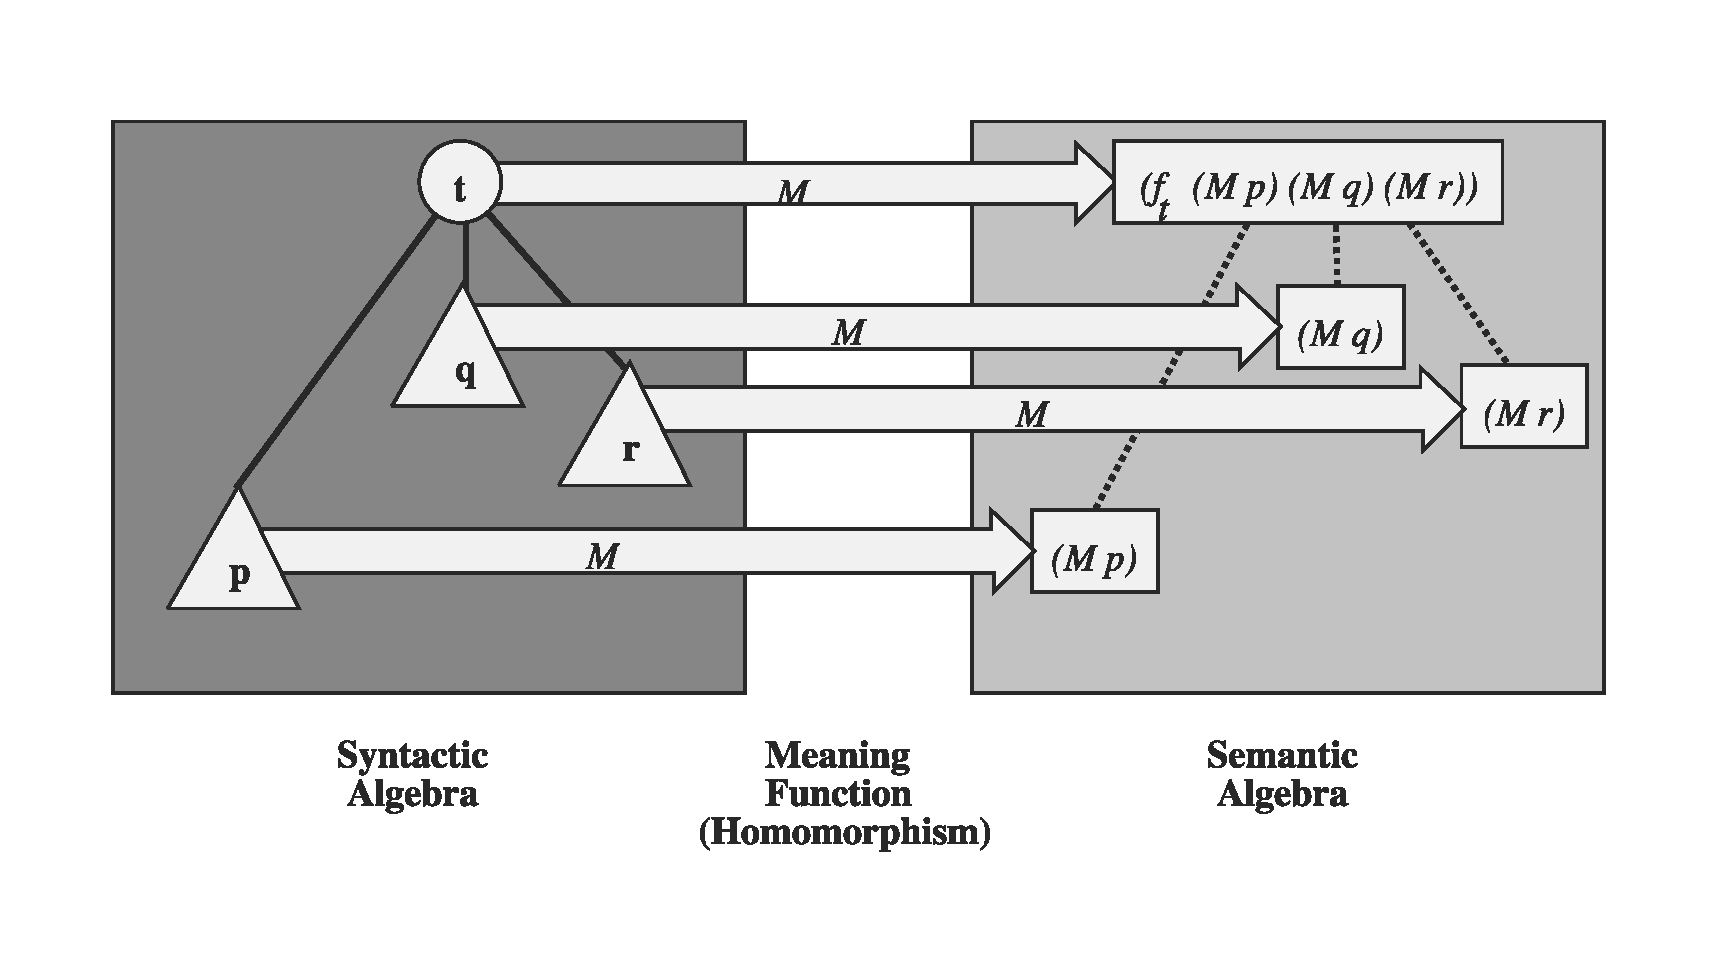
\includegraphics[width=125mm]{01/images/tpj-homo}
\end{figure}

\paragraph{Denotační sémantika} $Expr $ ::= $ Num \quad | \quad \bigtriangleup Expr \quad | \quad Expr \odot Expr$

\noindent Sémantická doména $N$

$$[\![n]\!] = n$$

$$[\![\bigtriangleup e]\!] = [\![\bigtriangleup]\!]([\![e]\!])$$

$$[\![\bigtriangleup]\!] = \lambda x.-x \quad \text{(např. unární mínus)}$$

$$[\![e_1 \odot e_2]\!] = [\![\odot]\!]([\![e_1]\!], [\![e_2]\!])$$

$$[\![\odot]\!] = \lambda x,y.x+y \quad \text{(např. plus)}$$

\subsection{Pevný bod funkce}
Jako pevný bod označujeme bod, který se v daném zobrazení zobrazí sám na sebe. Označuje se také jako samodružný bod. Například pevnými body funkce $f(x)=x^2-4x+6$, jsou čísla 2 a 3.

\begin{itemize}
\item bod, ve kterém platí $f(x) = x$
\item využívá se pro rekurzivní funkce
\item Y kombinátor v lambda kalkulu: \texttt{Y = $\lambda$y($\lambda$x.y(xx))($\lambda$x.y(xx))}
\end{itemize}

\priklad
Generující funkce faktoriálu fact = \texttt{$\lambda$F.$\lambda$X.if x==0 then 1 else F(decrement(X))}. Generující funkci dám do Y kombinátoru:

\begin{lstlisting}[
  mathescape,
  columns=fullflexible,
  basicstyle=\fontfamily{lmvtt}\selectfont,
]
Y fact =
       = $\lambda$f ($\lambda$x.y(xx))($\lambda$x.y(xx)) fact =
       = ($\lambda$x.fact(xx))($\lambda$x.fact(xx)) =
       = fact( ($\lambda$x.fact(xx) ($\lambda$x.fact(xx) ) =
       = fact(Y fact)
\end{lstlisting}

\noindent \texttt{Y fact} je pevný bod funkce, která počítá faktoriál.

\subsection{Vázání jmen}
Vázání jmen se vyskytuje v lambda kalkulu.
\paragraph{$\lambda$-kalkul} Je formální popis, který slouží jako základ pro funkcionální jazyky, takže všechny konstrukce v těchto jazycích jdou přepsat právě na $\lambda$-kalkul. Základní prvky $\lambda$-kalkulu jsou tři následující:
\begin{itemize}
\item \textbf{Proměnné} Obyčejné proměnné, tak jak je znáte z jiných jazyků, většinou se značí \texttt{x,y,z}.

\item \textbf{Abstrakce} Definice funkce – představte si např. funkci \texttt{f(x) = x+2}, tak přesně taková funkce se v $\lambda$-kalkulu zapíše takto: \texttt{$\lambda$x.x+2}. Část mezi $\lambda$ a tečkou jsou parametry funkce (zde máme pouze jeden parametr) a za tečkou se nachází tělo funkce.

\item \textbf{Aplikace} Volání funkce – když si vezmu naši funkci \texttt{f(x) = x+2}, tak ta se zavolá např. s argumentem 3 takto: \texttt{f(3)}. Funkce v $\lambda$-kalkulu se volají podobně, funkce se volá takto: \texttt{(f 3)}, tzn. nejdříve je uvedena funkce a poté její argumenty. Funkce f se v $\lambda$-kalkulu tedy zavolá takto: \texttt{($\lambda$x.x+2) 3}. Vysvětlení by mělo být už jasnější. Číslo 3 se dosadí za parametr \texttt{x} a přejde se do těla funkce, tam se ke 3 přičte 2 a výsledkem je 5.
\end{itemize}

\noindent Proměnná je v $\lambda$-výrazu \textit{vázaná}, pokud se jedná o parametr nějaké funkce, takže např. ve výrazu (\texttt{$\lambda$x.yx}) je \texttt{x} vázaná proměnná. Ostatní proměnné (v minulém příkladu \texttt{y}) jsou \textit{volné}. Proměnná se vždycky váže na nejbližsí lambdu vlevo, takže ve výrazu \texttt{($\lambda$x(($\lambda$x.x) w))} se proměnná \texttt{x} uprostřed výrazu váže na lambdu co je hned vlevo od ní a ne na tu úplně vlevo! Proměnná \texttt{w} je samozřejmě volná \cite{lambda}.

\begin{itemize}
\item Funkce, co mají jen vázané proměnné, vrátí při každém zavolání stejný výsledek. Funkce s volnými proměnnými jsou závislé na globálním kontextu.
\item Funkce, co mají jen vázané proměnné, se v $\lambda$-kalkulu nazývají kombinátory.
\end{itemize}

$$\texttt{(}\lambda\texttt{x.xy)}$$

$$\texttt{(}\lambda\texttt{x.x)(}\lambda\texttt{y.yx)}$$

\subsection{Stav programu}
Stav = proměnné v prostředí, proměnné mají typ, prostředí = množina všech proměnných, kontext (v handoutech $\Gamma$ (Gamma))
Čistě funkční jazyky (a matematika) jsou bezestavové, stavové výpočty mohou být reprezentovány jako iterace skrz stavy.

Čistě funkční jazyky (a matematika) jsou bezestavové, stav může být modelován jako iterace skrz stavy.
\example{Funkce na nalezení maxima z pole:}{
$$max:N* \rightarrow N$$

$$max(\langle a_1, \hdots, a_n \rangle) = loop(\langle a_1, \hdots, a_n \rangle,1,0)$$

$$loop: N* \times N \times N \rightarrow N$$

$$loop(\langle a_1, \hdots, a_n \rangle,c,m) = m \qquad \text{if} \quad c > n$$

$$loop(\langle a_1, \hdots, a_n \rangle,c,m) = loop(\langle a_1, \hdots, a_n \rangle,c+1,m) \qquad \text{if} \quad c \leq n \wedge a_c \leq m$$

$$loop(\langle a_1, \hdots, a_n \rangle,c,m) = loop(\langle a_1, \hdots, a_n \rangle,c+1,a_c) \qquad \text{otherwise}$$

\vspace{20px}
}

\paragraph{Monády} - struktury (typy), co reprezentují výpočet jako sekvenci kroků.

\subsection{Data programu}
Dělí se na \textbf{součiny}, \textbf{sumy} a \textbf{sumy součinů}.

\begin{itemize}[itemsep=0px]
\item Součiny
\begin{itemize}[itemsep=0px]
\item Positional data = N-tice, každý prvek může mít jiný typ
\item Sequence, List = pole
\item Named = třída
\item Nonstrict, stream = data, která se získají/vypočítají v okamžiku, kdy je potřeba (např. InputStream, odněkud se to vezme)
\end{itemize}

\item Sumy - Union v C, nadtypy v Javě.
\item Sumy součinů - Binární a ternální operátory, double dispatch.
\end{itemize} % TPJ
    %!TEX root=../oi-magistr-si.tex
\section[TPJ - Statická sémantika]{Statická sémantika: typy, polymorfní typy, typy vyššího řádu, rekonstrukce (inference) typů, abstraktní typy.}

Statická sémantika je řešena při překladu programu, zde jsou definovány a deklarovány jednotlivá pravidla a prvky programovacího jazyka. V těchto prvcích je zahrnuta jazyková konstrukce, její typy parametrů, význam příkazů a další prvky. Statická sémantika dále kontroluje statické typy a práci s tabulkou definovaných programových symbolů.

\begin{itemize}[itemsep=0px]
\item Staticky typované jazyky požadují uvedení datového typu u každé deklarace. Zde nelze deklarovat proměnnou, či funkci nebo objekt bez zadání datového typu.
\item Všechny typové kontroly jsou prováděny staticky při překladu. Už při překladu má být každé proměnné přiřazen datový typ.
\item Je možné daný datový typ přímo přetypovat. Přetypování především slouží k obcházení typových kontrol.
\item \textbf{Výhodou statického typování je lepší možnost odhalení typových chyb.}
\item Hlavní nevýhodou této metody je větší složitost programových konstrukcí, délka zdrojového kódu a tím i menší pružnost programovacího jazyka.
\item K nejčastěji vyskytovaným běhovým chybám patří přetečení datového typu.
\item Mezi neznámější zástupce staticky typovaných jazyků patří Java, Ada a jazyk C.
\end{itemize}

\subsection{Typy}

$$\Gamma \vdash e : A \qquad \text{\uv{$e$ je well-formed term typu $A$ v prostředí $\Gamma$}}$$

\begin{itemize}[itemsep=0px]
\item Typování
\begin{itemize}
\item \textbf{statické} - formálně specifikováno typovým systémem (judgements, typová pravidla, prostředí). Typová pravidla rozhodují platnost rozhodnutí (judgements) na základě jiných rozhodnutí o kterých je známo, že jsou platné.
\item \textbf{dynamické}
\end{itemize}
\item Typ je množina přípustných hodnot a operací s nimi.
\item \textbf{TopType}
\item \textbf{Type preservation} - zachování typu během přepisovací relace $\forall e,e'\in Expr:(\vdash e:t) \wedge e \rightsquigarrow e' \Rightarrow (\vdash e':t)$
\item \textbf{Progress} - když mám nějaký term v konfiguraci, tak pak to je buď finální konfigurace, nebo lze ještě nejméně jednou přepsat. Tzn. dobře otypovaný term neskončí ve \textit{stuck} stavu (stav, pro který není definován výstup). (důkaz lze udělat analýzou pravidel). $\forall e \in Expr: (\vdash e:t) \Rightarrow e \in (Num \cup Bool) \vee \exists e' \in Expr: e \rightsquigarrow e'$.
\item Type preservation + progress = \textbf{Soundness}. An argument is sound if and only if: \textit{The argument is valid} and \textit{All of its premises are true}. (i.e. All men are mortal. Socrates is a man. Therefore, Socrates is mortal.)
\item \textbf{Terminace} - důkaz např pomocí \textit{energie}, nadefinuji \uv{energii}, nadefinuji, že při každém přepsání se musí snížit.
\item \textbf{Determinismus} - programovací jazyk je deterministický právě tehdy když existuje právě jeden výstup pro každý pár \textit{programu} a \textit{vstupů}.
$\forall v,v' \in (Num \cup Bool): \forall e \in Expr : e \rightsquigarrow^* v \wedge e \rightsquigarrow^* v' \Rightarrow v = v'$. Platí to, protože platí konfluence relace.
\item \textbf{Konfluence} - \uv{strom vyhodnocování relace se rozdělí a pak se zase spojí}.
\end{itemize}

\subsection{Polymorfní typy}
Polymorfní typ je typ, jehož operace mohou být aplikovány na hodnoty jiného typu.
\begin{itemize}
\item \textbf{Rekurzivní} - používají se na zakodování seznamů a stromů, obsahují více hodnot stejného typu \url{http://en.wikipedia.org/wiki/Recursive_data_type}
\item \textbf{Univerzální} - generický typ, např. List<X>
\item \textbf{parametrický polymorfismus} - pomocí něj lze zapsat funkce jedním stylem a zároveň zachovat bezpečné typování. Tzn. funkce je zapsána genericky a umí zpracovávat vstupy bez ohledu na jejich typ. Typický příklad je třeba funkce append která se může zavolat s jakýmkoliv typem a správně se vyhodnotí. Není potřeba deklarovat \texttt{append :Integer} nebo \texttt{append:Bool}.
\item \textbf{ad-hoc polymorfismus} - jedna funkce může mít mnoho implementací na základě zpracování jednotlivých typů - přetěžování funkcí v Javě.
\end{itemize}



\subsection{Typy vyššího řádu}
\begin{itemize}
\item Product Type - např. tuple, 2 a více typů, 2 operandy ($A \times B$) \url{http://en.wikipedia.org/wiki/Product_type}
\item Union Type - datová struktura, která může udržovat více fixních typů \url{http://en.wikipedia.org/wiki/Tagged_union}
\item Function Type
\item Record Type - klasický objekt, který má fieldy
\end{itemize}

Jde o takzvané monády a debuggable functions (tohle je spíš možné využití). 

\paragraph{Monády} - umožňují řetězit procedury za pomocí čistě funkcionálního programování. Skládají se ze dvou operací a to bind a return(unit). 

\noindent \textit{\uv{In functional programming, a monad is a structure that represents computations defined as sequences of steps: a type with a monad structure defines what it means to chain operations, or nest functions of that type together. This allows the programmer to build pipelines that process data in steps, in which each action is decorated with additional processing rules provided by the monad.}}


\subsection{Rekonstrukce typů}
Schopnost z proměnné vyvodit její typ. Je to vlastnost některých silně staticky typovaných jazyků.

\noindent \textit{\uv{Type inference refers to the automatic deduction of the data type of an expression in a programming language. If some, but not all, type annotations are already present it is referred to as type reconstruction.}}

Například v csharpu, stačí místo typu psát klíčové slovo \texttt{var}.

\begin{verbatim}
var results = new Car();
// results je typu Car
\end{verbatim}

\subsection{Abstraktní typy}
Příkladem jsou Abstraktní třídy v Javě. Vyskytují se hlavně ve staticky typovaných jazycích.

Fronta, HashMapa, Množina (Set), Seznam (List), Zásobník (Stack), ...
 % TPJ
    %!TEX root=../oi-magistr-si.tex
\section[NUR - Teorie HCI]{Teorie HCI, kognitivní aspekty, způsoby interakce, speciální uživatelská rozhraní.}
\subsection{HCI - Human-Computer Interaction}

Human-Computer Interaction (česky interakce člověk - počítač) je průnikový \textbf{obor, který se zabývá fenoménem tvorby UI}. Zabývá se analýzou návrhu, vyhodnocování a zavádění interaktivních výpočetních systémů používaných lidmi a jevů, které interakci doprovázejí. Skládá se ze tří částí: \textbf{jedinec, počítač a způsob, jakým dohromady spolupracují}.

Cílem je návrh a vývoj prostředků a systémů, které jsou použitelné, efektivní, bezpečné a intuitivní. Dále se snaží přizpůsobit výměnu dat mezi lidmi a stroji tak, aby byla méně stresující a náchylná k nedorozumění.

\subsection{Kognitivní aspekty}
\begin{itemize}[itemsep=0px]
\item \textbf{kognitivní psychologie} zkoumá proces myšlení, učení a rozhodování
\item mentální model:
    \begin{itemize}[itemsep=0px]
    \item kognitivní struktura
    \item vnitřní reprezentace okolního světa, kterou si vytváříme v hlavě
    \item jak objekty určité třídy reagují s objekty jiné třídy, jak objekty v průběhu interakce mění své vlastnosti
    \item založeny na zkušenosti, mohou být nepřesné, neodpovídat zákonům fyziky
    \item lze je použít k predikci (kam dopadne hozený míč)
    \end{itemize}
\item kognitivní model uživatele - model, jak uživatel pracuje, na jehož základě se předpoví jeho chování (interakce s UI), výhody: nemusí se vytvářet prototypy, není nutné testování se skutečnými uživateli, vědecký základ pro návrh
\item estetika a efektivita kognitivních funkcí - důležitost vizuální podoby, atraktivní věci jsou použitelnější
\end{itemize}

\paragraph{Kognitivní teorie v HCI}
Modelování úkolů - metody KLM, GOMS
\begin{itemize}[itemsep=0px]
\item GOMS (Goals, Operators, Methods, Selectors) - popis struktury úloh, task rozpadlý do menších subtasků v hierarchicky přehledné síti,expert provádí UI operace
\item KLM (Keystroke-Level Model) - low-level verze GOMS, uživatelské operátory (K-keystroke, P-point, D-drawing, M-mental think), tabulkové časy pro každý operátor, každé operaci se přiřadí čas vykonání
\item Hick's Law - čas potřebný k rozhodnutí se, $n$ stejně pravděpodobných možností, průměrný čas výběru jedné z nich: $T = b \log_2(n + 1)$
\item Fitt's Law - předpovídá jak dlouho trvá uživateli vybrat cíl, vyhodnocení vstupních zařízení, pohyb k cíli o velikosti S ve vzdálenosti D: $T = a + b \log (\frac{D}{S} + 1)$, $a, b$ - konstanty závislé na zařízení
\item Model Human Processor / Human Information Processor Model - model lidského poznání vytvořený za použití teorií uvedených výše, modeluje, jak uživatel zachází s informacemi, perceptuální, kognitivní a motorický subsystém
\end{itemize}

\subsection{Způsoby interakce}
\begin{itemize}[itemsep=0px]
\item přímá manipulace - hry (značné implementační požadavky)
\item navigace (menu, odkazy) - web - není třeba si pamatovat příkazy jako CL, ale zabírá příliš místa na obrazovce
\item formuláře - web
\item příkazy - unix, první metoda komunikace člověk - PC, BNF, konečný automat
\item přirozený jazyk
\item nové typy interakce - mluva, gesta, eye-tracking, haptické (hmatová odezva) displeje
\end{itemize}

\subsection{Speciální UI}
\begin{itemize}[itemsep=0px]
\item mluvící systémy AI (Eliza, Cortana, Siri atd.)
\item multimodální - kombinování více vstupů
\item pokročilý vstup z klávesnice - pubtran se \uv{učí}
\item magnetický prsten - klikání, scrollování
\item haptická odezva
\item papírový mobil - ohýbací gesta
\item spolupráce telefonů např při sharování
\item multi-touch
\end{itemize}


\paragraph{Architektura UI}
Cíl: oddělení UI a aplikace, výběr možností prezentace informace uživateli, koordinace interakce, modifikovatelnost a přenositelnost. Interaktivní systém poskytuje tři funkce (vrstvy):
\begin{itemize}[itemsep=0px]
\item prezentační (UI)
\item dialogovou (komunikace s uživatelem)
\item aplikační (vlastní účel SW systému)
\end{itemize}
\textbf{Monolická architektura} = všechny části v jednom

\paragraph{Seeheim model}
\href{http://centurion2.com/SEHomework/UserInterfaceDesign/UserInterfaceDesign.php#SeeheimModel}{URL}
sémantická vazba je často pomalejší, přímá vazba mezi aplikační a prezentační vrstvou regulovaná dialogem umožní okamžitou odezvu (switch).

Výhody:oddělená prezentační vrstva podporuje přenositelnost a modifikovatelnost, oddělená aplikační vrstva dovoluje modifikace aplikace beze změny UI, oddělená dialogová část umožňuje změnit uživatelskou interakci beze změny prezentační části.
Nevýhody: řada modifikací se promítá do všech částí, komplikované sémantické vazby.

$$lexical \qquad - \qquad syntactic \qquad - \qquad semantic$$
$$\text{Prezentace} \qquad - \qquad \text{Dialog} \qquad - \qquad \text{Aplikace}$$ % NUR
    %!TEX root=../oi-magistr-si.tex
\section[NUR - Metody návrhu, uživatelské a konceptuální modely]{Metody návrhu, uživatelské a konceptuální modely}

\begin{figure}[h!]
\centering
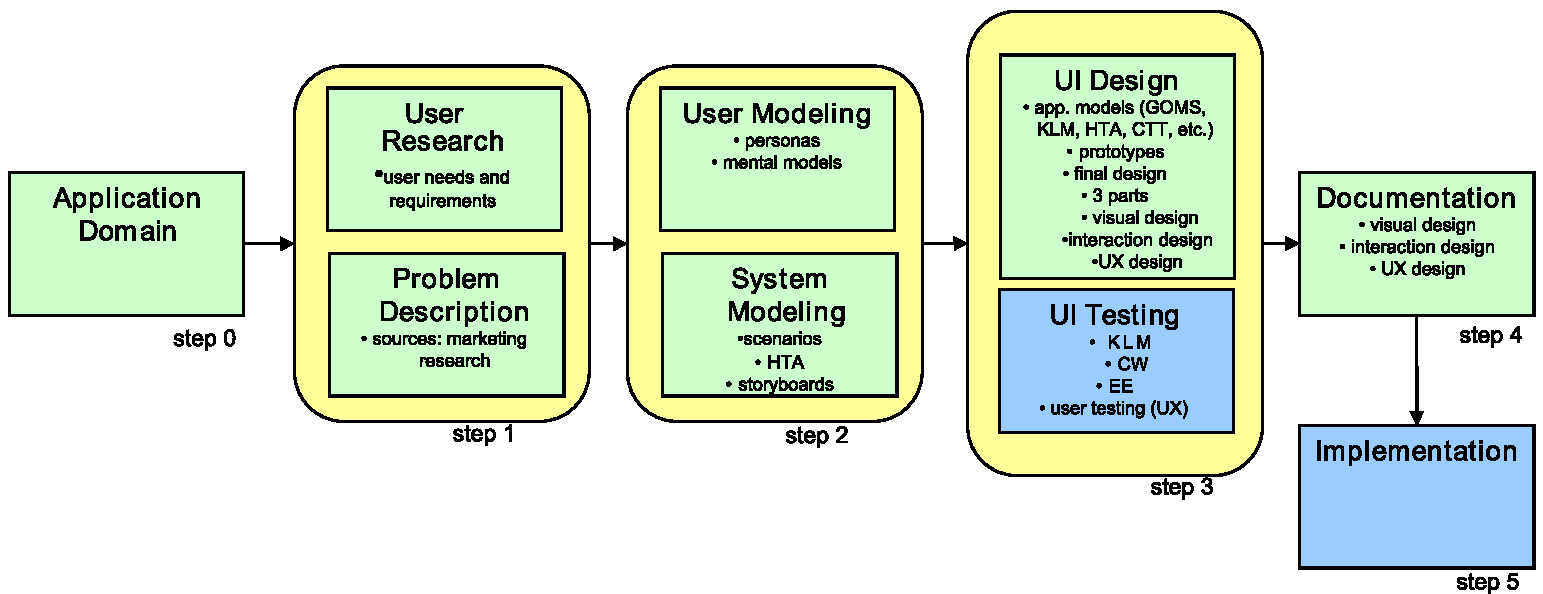
\includegraphics[width=125mm]{04/images/hci}
\end{figure}

\paragraph{Cyklus tvorby UI}
\begin{itemize}[itemsep=0px]
\item Návrh - porozumění uživateli (cílová skupina) a jeho potřebám
\begin{itemize}[itemsep=0px]
\item \textbf{analýza úlohy} - výkonnost software, hardware, uživatele při provádění úlohy, co uživatelé dělají, co k tomu potřebují za nástroje, co potřebují vědět, metoda: HTA
\item popis průběhu dialogu, slouží k následující implementaci UI
\end{itemize}
\item Implementace - prototypování
\item Vyhodnocení - hodnocení prototypu ve spolupráci s uživateli (kvalitativní \&
kvantitativní)
\item další iterace...
\end{itemize}

\paragraph{Analýza}
\begin{itemize}[itemsep=0px]
\item specifikace aktivit, které systém bude dělat
\item specifikace uživatelů - ti, kteří aktivity budou dělat
\item volba formy řešení - forma UI, SW podporující UI, OS, systémové požadavky, HW
\end{itemize}

\paragraph{Uživatel}
\begin{itemize}[itemsep=0px]
\item Uživatelské požadavky - Obecné požadavky: fyzické, kognitivní, sociální. Mohou být také specifické požadavky, které se vztahují přímo k problémmu.
\item Modely uživatele - KLM (Keystroke-level model), persony
\end{itemize}

\paragraph{Principy použitelného návrhu (usable design)}
\begin{itemize}[itemsep=0px]
\item jednoduché a přirozené dialogy v jazyku uživatele
\item konzistentnost akcí, příkazu, layoutu, terminologie
\item minimalizovat paměťovou zátěž uživatele - rozpoznávání je snazší než
vzpomínání
\item zpětná vazba
\item kontrola vstupu
\item snadné vrácení akcí - podpoří chuť experimentovat
\item výrazně značená ukončení - uživatel se nesmí ocitnout v pasti
\item zkratky - rychlé provedení časté akce pro zkušené uživatele
\item robustní systém poskytující snadno ovladatelné prostředky k nápravě chyb
\item užitečná nápověda a dobrá dokumentace (hledána v kritických situacích)
\end{itemize}

\paragraph{Terminologie}
\begin{itemize}[itemsep=0px]
\item Goal - to čeho chceme dosáhnout
\item Task - posloupnost aktivit, která dá \textit{goal}
\item Action - krok nebo akce - část \textit{tasku}
\end{itemize}

\subsection{Specifikace požadavků}
\begin{itemize}[itemsep=0px]
\item HTA (Hierarchical task analysis) - dekompoziční strom, kde je \textit{goal} zakreslen do postupně se rozpadajících menších \textit{tasků}. (CTT\footnote{Concurrent Task Tree} - strom s operátory a symboly)
\item Storyboard - série snímků a skeč§ (\uv{komiks} popisující \textit{goal})
\item Scénáře - jednoduché výpravné příběhy průběhu úkoli \textit{\uv{Uživatel napíše všechny účastníky akce, poté systém zkontroluje zda je vše vyplněno v pořádku a vytvoří událost...}}.
\item Případy užití - popis interakce člověka se systémem.
\end{itemize}

\subsection{Uživatelský průzkum}
Získávání informací o budoucích uživatelech systému, jejich \textbf{potřeby, zvyky , zkušenosti a dovednosti}.

\begin{itemize}[itemsep=0px]
\item \textbf{kvalitativní} - menší vzorek lidí, více informací, rozhovor, etnografické (pozorování chování) pozorování
\item \textbf{kvantitativní} - více lidí, méně informací, průzkumy, testy, pozorování
\item kombinovaný
\end{itemize}

\paragraph{Persona}
Detailně popsaný hypotetický uživatel reprezentující nějakou uživatelskou skupinu. Je založen na nasbíraných informacích. Nevýhody mohou být: nekonzistentní uživatel, představování si sama sebe jako uživatele.

\paragraph{Metody sběru dat}
\begin{itemize}[itemsep=0px]
\item pozorování - introspekce (sebepozorování) - zahrnuje kognitivní průchod, extrospekce
\item rozhovor - strukturovaný vs. volný, být neutrální a zvědavý (30-90 min), přímé otázky, žádná anonimita, vliv tazatele
\item dotazování (průzkum) - jednoduché otázky, používat rozsahy, neopakovat otázky, lidé lžou (chtějí vše, levně a ihned)
\item experiment
\end{itemize}

\subsection{Modely pro návrh UI}
\textbf{Konceptuální} model (design model) znamená to, jak to je navrženo. \textbf{Uživatelský} model (user model) značí co uživatel očekává. Nesoulad modelů vede k pomalému provádění úloh, chybám a frustraci

\paragraph{Mentální model} Uživatelovo porozumění jak se objekty chovají a jak akce prováděné přes UI ovlivňují jejich chování získané na základě zkušeností. Očekávané struktury a chování (menu, ukládání souborů, zpětná vazba, interpretace akcí). Vědomé i podvědomé procesy, které obsahují aktivaci obrazů a analogií. Hluboké a mělké modely (řízení auta vs. fungování auta).

UI musí prezentovat model vizuálně, mapování reálných prvků na rozhraní. Dobrý konceptuální model zahrnuje:
\begin{itemize}[itemsep=0px]
\item dostupnost funkcí (affordances)
\item návaznost (kauzalita)
\item omezení (constraints)
\item mapování jednotlivých kroků na akce
\item vzory chování cílových uživatelů
\end{itemize}
 % NUR
    %!TEX root=../oi-magistr-si.tex
\section[NUR - Formální popis uživatelských rozhraní]{Formální popis uživatelských rozhraní}

\paragraph{HTA (Hierarchical task analysis)} Dekompoziční strom, kde je nějaký cíl (úloha) zakreslen do postupně se rozpadajících menších podúloh. Používá se ve fázi návrhu UI pro popis vzájemného uspořádání podúloh.

\begin{figure}[h!]
\centering
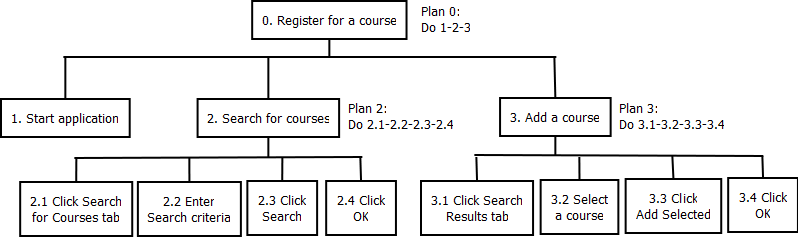
\includegraphics[width=130mm]{05/images/hta}
\end{figure}

\paragraph{CTT (Concurrent Task Tree)} Podobný strom jako HTA, ale s operátory a symboly. Úloha přihlášení: vyplním uživatelské jméno a zároveň heslo, pak je mi umožněho se připojit.

\begin{figure}[h!]
\centering
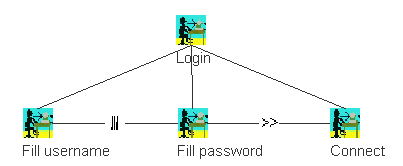
\includegraphics[width=100mm]{05/images/ctt}
\end{figure}
\vspace{-15px}
\begin{itemize}[itemsep=0px]
\item Enabling T1 $>>$ T2
\item Disabling T1 [> T2
\item Interruption T1 |> T2
\item Choice T1 [] T2
\item Iteration T1* nebor T1$_{n}$
\item Concurrency T1 ||| T2
\item Optionality [T]
\end{itemize}


\paragraph{Storyboard} Série snímků a skečů (\uv{komiks} popisující nějakou úlohu).

\paragraph{Scénáře} Jednoduché výpravné příběhy průběhu úkolu

\textit{\uv{Uživatel napíše všechny účastníky akce, vyplní místo a datum konání. Systém poté zkontroluje zda je vše vyplněno v pořádku a vytvoří událost.}}.

\paragraph{Případy užití} Popis interakce člověka se systémem..

\paragraph{Keystroke-Level Model (KLM)}
Cílem je vypočítat čas potřebný pro provedení úlohy
Operátory:
\begin{itemize}[itemsep=0px]
\item stisk klávesy (\textbf{K}eystroke) - určený rychlostí psaní
\item ukázat na cíl na displeji (\textbf{P}ointing) - určeno pomocí Fitt's Law
\item položit ruku na vstupní zařízení (\textbf{H}oming) - odhad měřením
\item mentální příprava akce (\textbf{M}ental preparation) - odhad měřením, heuristika pro předřazení
\item čas reakce systému (\textbf{R}eaction)
\end{itemize}
Jsou časové odhady (tabulkové) pro každý operátor. Předpokládá provádění úloh bez chyby, předpovídá jen efektivitu, ignoruje paralelní zpracování, prokládání úloh, mentální zátěž, plánování a řešení úlohy (\uv{přemýšlecí} čas, uvažovány jsou jen holé akce)


\paragraph{Goals, Operators, Methods, Selection Rules (GOMS)}
Nejznámější používaná metoda. Složky:
\begin{itemize}[itemsep=0px]
\item \textbf{Goals} - cíle z hlediska úmyslů koncového uživatele
\item  \textbf{Operators} - elementární perceptuální, kognitivní a motorické akce s fixním časem
bez ohledu na kontext
\item \textbf{Methods} - posloupnost operátorů a podcílů
\item \textbf{Selection rules} - if-then pravidla určující, kterou metodu použít
\end{itemize}

Předpokládá provádění úloh bez chyby, úlohy musí mít přesně definovaný cíl, nemodeluje proces řešení problému, chování uživatele

\paragraph{Dialog modeling}
Z HTA máme představu o posloupnosti kroků, potřebujeme popsat, jak při provádění kroků spolu budou komunikovat uživatel a počítač - jak bude probíhat dialog
\begin{itemize}[itemsep=0px]
\item textové (gramatiky, produkční pravidla, událostní algebry)
\item diagramy - (STN, PN, flowcharts, JSD)
\end{itemize}

\paragraph{State Transition Networks (STN)}
Varianta konečných automatů, konečný počet stavů a přechodů mezi nimi, automat se nachází v pravě jednom stavu (stavy jsou disjunktní). Reakcí na každý uživatelský vstup je přechod z daného stavu do nového stavu. Stav má přiřazenou akci, musí být odlišitelný od jiných stavů, charakterizován vstupy, které k němu vedou. Přechod mezi stavy může být vázán podmínkou, lze k nim přiřazovat popis akcí.
\begin{itemize}[itemsep=0px]
\item[$+$] model UI, se kterým lze experimentovat
\item[$+$] možnost automatického nebo poloautomatického vytváření UI
\item[$+$] kontrola vlastností (úplnost, reversibilita, dostupnost, nebezpečné stavy - ukončení bez uložení)
\item[$-$] některá zařízení mohou mít velká množství stavů
\end{itemize}

\begin{figure}[h!]
\centering
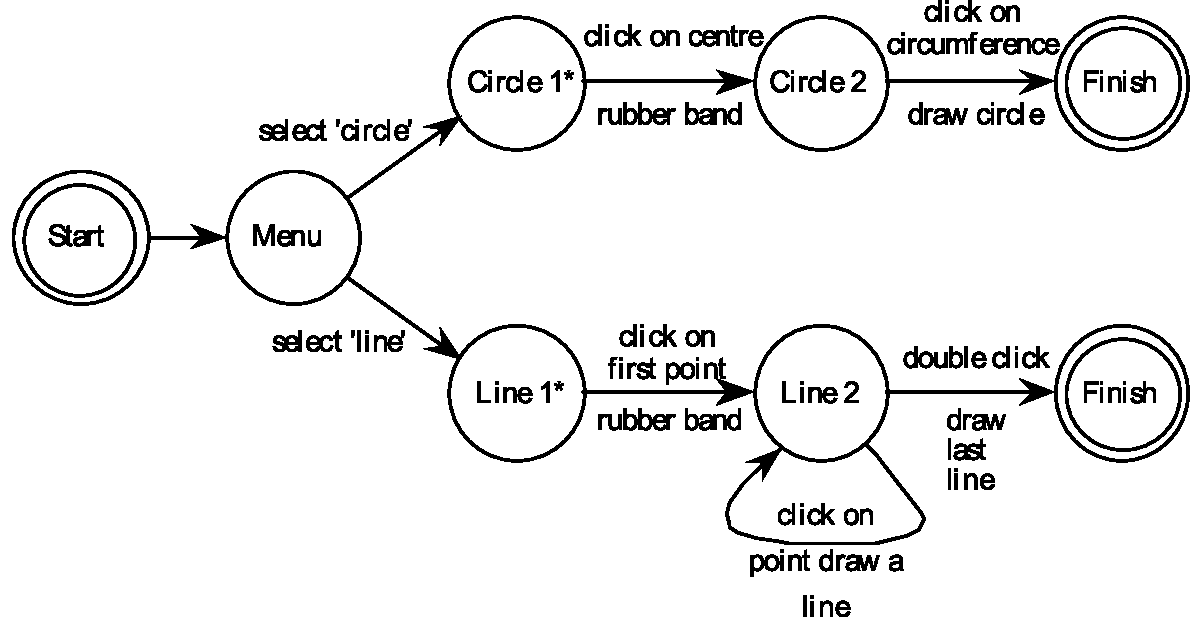
\includegraphics[width=130mm]{05/images/stn}
\end{figure}

\textbf{hierarchické STN} - varianta pro popis složitých dialogů, obsahuje sub-dialogy (vnořené další sítě).

\paragraph{Petriho sítě (PN)} Oproti STN mají synchronizaci - pokračování při splněné podmínce % NUR
    %!TEX root=../oi-magistr-si.tex
\section[NUR - Prototypování uživatelských rozhraní]{Prototypování uživatelských rozhraní}
Prototypování se dělá v ranných fázích návrhu. Rozděluje na \textbf{Low-Fidelity} a \textbf{High-Fidelity} prototypování.

\subsection{Low-Fidelity}
První náčrtky rozhraní. Jsou to víceméně narychlo načmárané skicy bez detailů, spiše jde o základní rozvržení (layout) prvků, žádná interakce. Typicky skicy na papíru nebo na elektronických prototypovacích SW (není na finálním zařízení). Je to spíše o rychlém zhodnocení nápadů, které jsou převedeny na papírový prototyp.

\begin{itemize}[itemsep=0px]
\item velké množství nápadů/alternativ
\item krátká doba vývoje - hodiny/dny
\item neběží na finálním zařízení
\item bez interakce
\item testování v laboratoři
\end{itemize}

\vspace{20px}

\begin{figure}[h!]
\centering
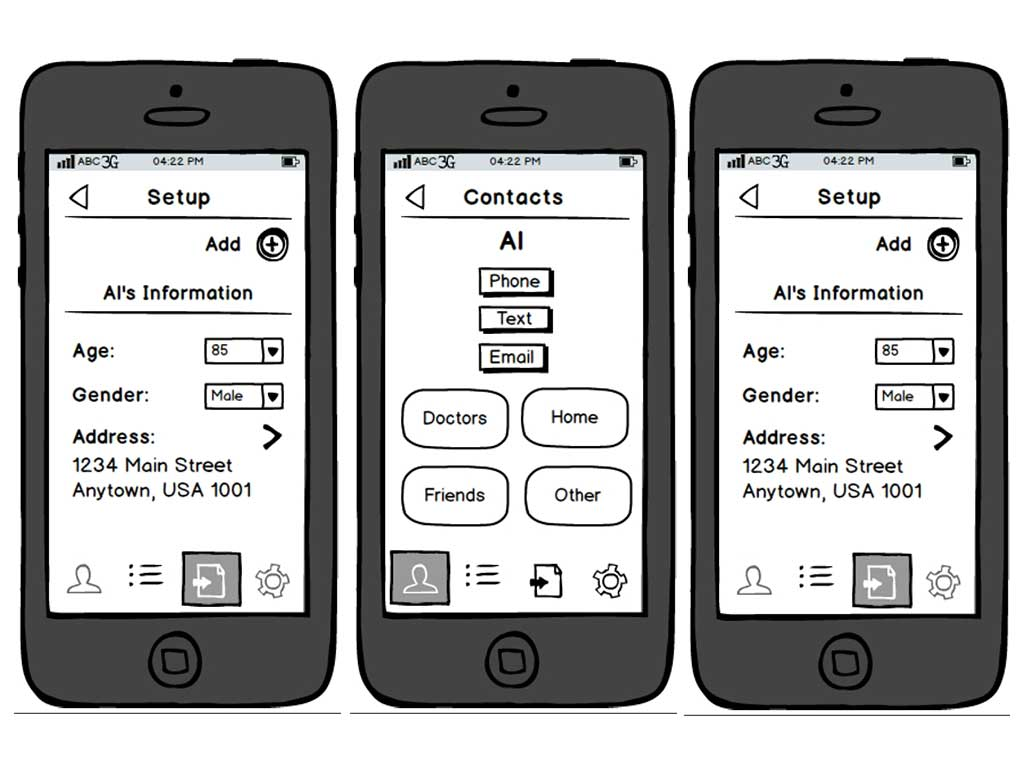
\includegraphics[width=110mm]{06/images/lofi}
\end{figure}

\vspace{20px}

Např. prototypování mobilní app. Vytvoří se několik papírků, každý popisuje krok aplikace. Interakce v podobě fiktvního klikání na papír, dochází k výměně papírků (změna stavu) a tím dochází k fiktivní interakci.

\subsection{High-Fidelity}
Iluze finálního vizuálního (i interagujícího) návrhu. Vzhled by měl následovat \textit{guidelines} cílové platformy (MS Windows, Android, iOS, ..). Prototyp již ve funkční podobě na cílovém zařízení, např. na telefonu. Interakce realizována jakoby to byla již výsledná aplikace, ovšem logika ještě nemusí být implementována (dummy data, \textit{Wizard of Oz}, atd.,). Hlavní části

\begin{itemize}[itemsep=0px]
\item málo alternativ (pokud vůbec nějaké jsou)
\item dlouhá doba vývoje - dny/týdny
\item dostupné na finálním zařízení
\item podoba a interakce téměr podobná té finální
\item testování v laboratoři a v \uv{terénu} (v reálných podmínkách využití)
\end{itemize}

\begin{figure}[h!]
\centering
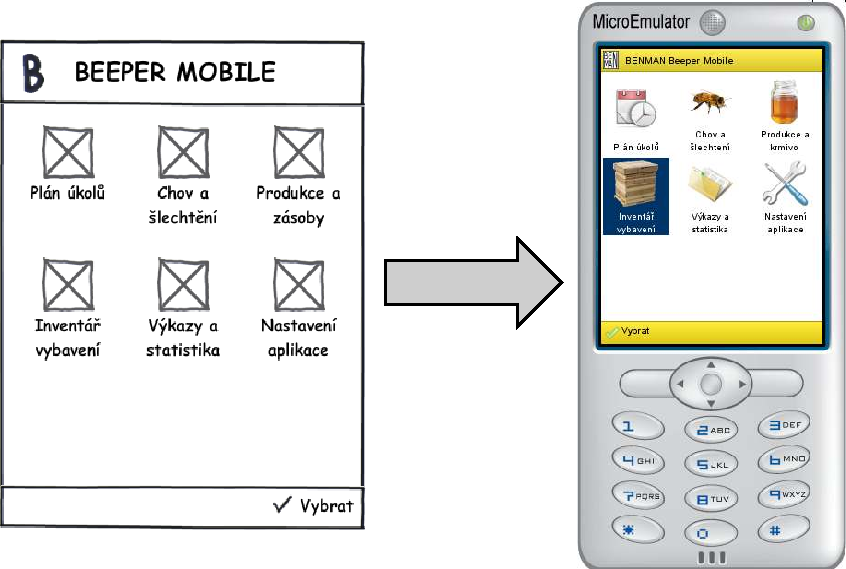
\includegraphics[width=80mm]{06/images/hifi}
\end{figure}

\paragraph{Problémy s prototypováním}
\begin{itemize}[itemsep=0px]
\item U lo-fi prototypů dochází ke skipování hlubokých (detailních) uživatelských požadavků
\item user confusion: hi-fi prototyp vs. finální aplikace
\item drahé a žrout času (speciálně hi-fi)
\end{itemize} % NUR
    %!TEX root=../oi-magistr-si.tex
\section[OSP - Open source,git,lincence]{Techniky správy a organizace rozsáhlých softwarových projektů. Nástroje pro správu verzí zdrojových kódů, sledování chyb, pro automatické generování dokumentace a podporu orientace v rozsáhlých projektech. Způsoby komunikace mezi vývojáři navzájem a i s uživateli. Systémy pro sledování a řešení chyb a uživatelskou podporu. Open-source licence a z nich vyplývající práva a licence. Postup začlenění úpravy (patche) do velkého open-source projektu (např. Linuxové jádro)}

\paragraph{Motivace pro verzování zdrojového kódu} Verzování kódu umožňuje sdílení kódu mezi vývojáři, zálohování, paralelní vývoj v několika souběžných větvích, vrácení se ke konkrétní revizi kódu, zjištění autorství nebo zobrazení statistik. Bez verzovacího systému není možná efektivní spolupráce více vývojářů na jednom projektu. Verzovací systém přináší výhody i v případě, že na projektu pracuje jediný vývojář.

\subsection{Nástroje pro správu verzí kódu}
GIT je distribuovaný SCM\footnote{Source Code Management} od Linuse Torvaldse. Každá working copy je zároveň repozitář, nezávislé na centrálním serveru. Spoustu operací jako merge, branch,... lokálně. Commity jsou hash celé historie vedoucí ke commitu. Nevýhoda: častější konflikty Subversion (SVN) je centrální SCM, ale rozšířený = dobré nástroje, GUI atd. Míň konfliktů, ale závislost na serveru. CVS podobné SVN ale starší, nevýhody: drahé branchování, problémy s Unicode, netrackuje přejmenovávání a mazání souborů.

\subsection{Nástroje pro sledování chyb (bug trackers)} Jsou nástroje (např. bugzilla), které sledují a soustřeďují nalezené chyby. Každá chyba má vypsaný svůj \textit{ticket}, ve kterém jsou veškeré informace k chybě: popis, priorita, reportující osoba, přiřazená osoba, návrh úpravy (např. v podobě patche).

\subsection{Nástroje pro automatické generování dokumentace}
Javadoc generuje HTML dokumentaci z komentářů v Java kódu, Doxygen je multijazykový generátor dokumentace z kódu, Enterprise Architect umí generovat UML diagramy z kódu.

\subsection{Systémy pro spolupráci mezi vývojáři}
GitHub je populární sociální platforma pro vývojáře na hosting a spolupráci open-source projektů založený na použítí Gitu, Trac je project management systém v Pythonu, který si můžete nasadit na vlastní server, obsahuje wiki, bug tracking, time management, etc. Spíše pro menší projekty. JIRA je SaaS systém podobný Tracu se spoustou pluginů, hodí se pro větší projekty.


\begin{itemize}[itemsep=0px]
\item Google Groups a podobné mailing listy mohou také sloužit k podpoře.
\item wiki stránky
\item fóra
\end{itemize}

\subsection{Licence}
Svobodný software je software, který respektuje svobodu svých uživatelů a poskytuje jim čtyři základní svobody, které svobodný software definují (publikace FSF 1986):

\begin{enumerate}[itemsep=0px]
\item svoboda používat program za jakýmkoliv účelem
\item svoboda zkoumat a upravovat program (předpokladem je přístup
ke zdrojovému kódu)
\item svoboda šířit původní verzi programu
\item svoboda šířit upravenou verzi programu
\end{enumerate}

\begin{itemize}[itemsep=0px]
\item \textbf{Komerční software} – licence daná smluvními podmínkami jež uživatel potvrzuje při nákupu SW
\item \textbf{Freeware} – zdarma, většinou bez zdrojových kódů, podmínky mohou omezovat další šíření, (komerční) použití, zkoumání
\item \textbf{Shareware} – jako freeware, ale specifikuje pro které druhy použití je nutné pořídit placenou verzi
\item \textbf{Permisivní} (akademické) licence (BSD, MIT) – povolují použití/integraci do komerčního SW, vyžadují jen uvádění autora/ů (to je i instituce)
\item \textbf{Copyleftové} (reciproční) licence (GPL, LGPL, MPL)
vyžadují zahrnutí uživatelů do okruhu oprávněných osob k právu nakládat s dílem (modifikovat ho a šířit za stejných podmínek)
\end{itemize}
\paragraph{Upozornění:} Definice open-source nevyžaduje \textit{copyleft}.

\subsubsection{BSD (Berkeley Software Distribution)}
BSD licence je licence pro svobodný software, mezi kterými je jednou z nejsvobodnějších. Umožňuje volné šíření licencovaného obsahu, přičemž vyžaduje pouze uvedení autora a informace o licenci, spolu s upozorněním na zřeknutí se odpovědnosti za dílo.

\subsubsection{MIT License}

Licence podobná BSD licenci umožňuje se software nakládat téměř libovolně (používat, kopírovat, modifikovat, slučovat, publikovat, distribuovat či prodávat), jedinou podmínkou je zahrnutí textu licence do všech kopií a odvozenin software.

\subsubsection{Apache License}
Stejné myšlenkové základy jako licence BSD a MIT. Výslovná zmínka možnosti šířit odvozená díla pod jinou kompatibilní licencí.

\subsubsection{GNU GPL (GNU General Public License)}

GPL je nejpopulárnějším a dobře známým příkladem silně copyleftové licence, která vyžaduje, aby byla odvozená díla dostupná pod toutéž licencí. 

GNU General Public License. Software šířený pod licencí GPL je možno volně používat, modifikovat i šířit, ale za předpokladu, že tento software bude šířen bezplatně (případně za distribuční náklady) s možností získat bezplatně zdrojové kódy. Toto opatření se týká nejen samotného softwaru, ale i softwaru, který je od něj odvozen. Na produkty šířené pod GPL se nevztahuje žádná záruka. Licence je schválená sdružením OSI a plně odpovídá Debian Free Software Guidelines.

V rámci této filosofie je řečeno, že poskytuje uživatelům počítačového programu práva svobodného softwaru a používá copyleft k zajištění, aby byly tyto svobody ochráněny, i když je dílo změněno nebo k něčemu přidáno. Toto je rozdíl oproti permisivním licencím svobodného softwaru, jejímž typickým případem jsou BSD licence

\subsubsection{GNU LGPL (GNU Lesser General Public License)}

Lesser/Library GPL. Licence je kompatibilní s licencí GPL. Pod touto licencí se šíří zejména knihovny, protože narozdíl od licence GPL umožňuje nalinkování LGPL knihovny i do programu, který není šířen pod GPL.

\subsubsection{MPL (Mozilla Public License)}
Mozilla Public License. Základním elementem pokrytým licencí je každý jednotlivý zdrojový soubor. Autor takového souboru umožňuje komukoliv používat, měnit a distribuovat jeho zdrojový kód (i jako součást většího díla). Každá změna původních souborů je krytá licencí, tzn. musí se tedy zveřejnit. To samé platí pokud přenesete část původního souboru do nového souboru, tj. celý nový soubor je pak nezbytné zveřejnit. Pokud vytváříte nový produkt přidáním nových souborů, můžete pro tyto nové soubory použít libovolnou licenci. Binární verze lze licencovat libovolně, pokud to není výslovně v rozporu s MPL (zákaz distribuce zdrojů). Produkty pod touto licencí jsou distribuované jak jsou ("as is"), tj. bez záruk libovolného druhu.

\subsubsection{CreativeCommons}
Je license vhodná pro jakýkoli obsah, nejenom pro software. Do license si člověk může dát 1-4 z těchto atributů:
\begin{itemize}[itemsep=0px]
\item Attribution - nutno uvést autora originálního projektu
\item Noncommercial - možno upravovat jenom pro nekomerční účely
\item NoDerivatives - možno pouze kopírovat dané dílo, ale nikoliv ho upravovat
\item Share-alike - znamená virální copyleft
\end{itemize}


\subsection{Kontribuce do projektu}
TODO
% http://git-scm.com/book/cs/v1/Distribuovaný-charakter-systému-Git-Přisp%C3%ADván%C3%AD-do-projektu
 % OSP
    %!TEX root=../oi-magistr-si.tex
\section[OSP - Přenositelnost, multiplatformnost]{Požadavky a pravidla pro tvorbu přenositelného kódu. Organizace projektů a struktura operačních systémů pro zajištění přenositelnosti mezi různými platformami (OS, CPU). Vnitřní a vnější reprezentace dat, převody mezi nimi, vztah k síťovým protokolům (endianing, serializace atd.)}

\subsection{Požadavky a pravidla pro tvorbu přenositelného kódu}
Při realizaci softwarových systémů často nemůžeme zanedbat cílovou hardwarovou architekturu stroje a musíme psát kód tak, aby jej bylo možné snadno upravit (ideálně pouze rekompilovat) pro běh na jiných platformách. V okamžiku kdy je nutné přímo interagovat s některou hardwarovou komponentou počítače (řídící jednotky, SCADA systémy, $\hdots$), se dostáváme až na úroveň, kdy musíme řešit věci, jako uspořádání bytů v proměnné apod. K základním požadavkům na přenositelnost zdrojového kódu patří:

\begin{itemize}[itemsep=0px]
\item psát čistě a používat jen to, co je jazykem deklarováno,
\item pokud je to možné používat pouze standardizovaná API - POSIX, IEEE Std. 1003.1,
\item nepředpokládat pořadí byte/char ve slovech - little versus big endian,
\item nepředpokládat počet bitů v adresační jednotce (používat stdint.h - int32\_t, $\hdots$),
\item psát kód proti knihovnám a nikoliv přímo proti konkrétním voláním služeb operačního systému (konkrétním makrům, číslům volání, atd.).
\end{itemize}

\subsection{Organizace projektů a struktura operačních systémů pro zajištění přenositelnosti mezi různými platformami (OS, CPU)}

Aby bylo možné snadno přenášet projekty mezi různými operačními systémy a jejich verzemi a hardwarovými architekturami, bylo definováno několik standardů a vyvinuto několik nástrojů, které mají tuto přenositelnost usnadnit:
\paragraph{POSIX} - Portable Operating System Interface - standardy IEEE 1003 a ISO/IEC 9945 - definuje, co by měl poskytovat operační systém, jaké příkazy, jaké vlastnosti - na základě tohoto standardu je potom poměrně snadné převádět projekty mezi různými distribucemi Linuxu, UNIXY, atd. (uvádí se, že to je mnohdy jednodušší než převod projektů mezi různými verzemi Windows).

\paragraph{Filesystem hierarchy standard (FHS)} - dokument popisující, co má být ve kterém adresáři v linuxové distribuci, mezi typické adresáře patří
\begin{itemize}[itemsep=0px]
\item \texttt{/usr/bin} - binární programy (platformně závislé)
\item \texttt{/usr/local} - prefix do kterého je instalován software lokální pro tento stroj
\item \texttt{/usr/share} - sdílené (na hw platformě nezávislé) zdroje - často může být tento systém sdílen mezi různými stroji (např. pomocí NFS)
\item \texttt{/usr/lib} - knihovny (platformně závislé)
\item FHS popisuje, co by měl/neměl který adresář správně obsahovat
\end{itemize}

\subsection{Kompilace GNU balíků}
Nejrozšířenějším nástrojem pro kompilaci GNU balíků je systém Autotools. Tento systém se skládá z více nástrojů. Mezi hlavní a nejdůležitější patří:
\begin{itemize}[itemsep=0px]
\item m4, aclocal, autoheader
\item autoheader
\item autoconf
\item automake
\end{itemize}

Tyto nástroje zpracovávají vstupní soubory, které obsahují informace o projektu, závislostech, požadavcích na cílovou platformu atd. Jedná se zejména o soubory: \texttt{Makefile.am}, \texttt{configure.ac}, \texttt{config.h.in}.

Proces sestavování (build) softwarového balíku se dělí na část, která probíhá u vývojáře (vyžaduje ke svému běhu větší množinu nástrojů) a část, kterou spouští klient.

\subsection{Portace kódu a křížový překlad}
Většinou není nutné, aby každý uživatel kompiloval software ze zdrojových kódů. Je možné dodávat konkrétní verzi zkompilovanou pro cílovou platformu. Pro sestavení programu se používá build toolchain (v případě použití GCC se označuje jako GNU Tool Chain). Ten zahrnuje jednak vlastní kompiler (např. GCC - GNU Compiler Collection) a dále nástroje pro vytváření knihoven, linker atd.

Tento toolchain může kompilovat kód pro různé platformy. Na základě toho rozeznáváme native toolchain a cross-compiling toolchain (výsledné binární soubory běží na platformě toolchainu nebo na jiné platformě).

\begin{figure}[h!]
\centering
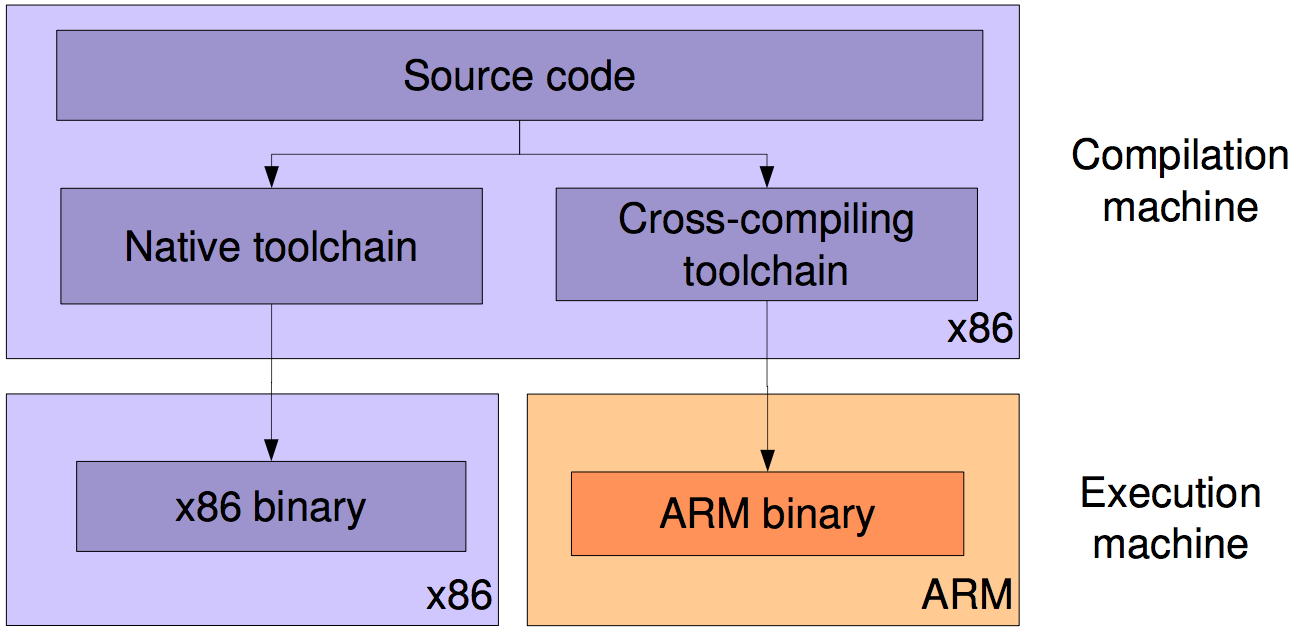
\includegraphics[width=130mm]{08/images/portace-kodu}
\end{figure}

\subsection{Konverze vnitřních a vnějších/síťových formátů dat}

Na to je tam slajd.. endianita, rozsah cisel
https://rtime.felk.cvut.cz/osp/prednasky/osp-hw-and-porting.pdf

\begin{itemize}[itemsep=0px]
\item little endian/big endian
\item textové formáty: XML, HTML, SOAP, JSON
\item XDR (external data representation) - nezávislý na arch. systému, od roku 1995 IETF standard
\item RPC, CORBA
\item padding - zarovnávání packetů
\end{itemize} % OSP
    %!TEX root=../oi-magistr-si.tex
\section[AOS - SOA]{Co je to architektura zaměřená na služby (SOA)? Základní pojmy, vztah k objektově orientované architektuře. Konceptuální model a formalismy pro modelování SOA.}

\subsection{Architektura zaměřená na služby (SOA)}
SOA je model softwarové architektury, kde byznys funkcionalita je logicky oddělena (grupována).

\begin{itemize}[itemsep=0px]
\item \textbf{sada návrhových principů} používaných během vývoje systému a integrace.
\item SOA je styl návrhu takových aplikací, které jsou složeny z vícero odlišných částí (poskytující funkcionalitu jako služby jiným aplikacím), které mají definované jednoduché rozhraní.
\item SOA nabízí množinu služeb, které mohou být použity v různých business doménách
\item způsob, jak spolu mohou dvě \textbf{distribuované aplikace} komunikovat, i když běží na různých \textbf{platformách} a \textbf{technologiích}
\item definuje \textbf{rozhraní} ve smyslu protokolů (WSDL, XML, HTTP, UDDI, SOAP) a funkcionalit
\item dodržuje zásady loose coupling jak mezi jednotlivými službami, tak mezi službou a vrstvou, která leží pod ní
\item odděluje funkčnost do nezávislých menších jednotek (nebo services), které jsou dostupné na síti
\end{itemize}

\textit{\uv{SOA is a style of architecting applications in such a way that they are composed of discrete software agents that have simple, well defined interfaces and are orchestrated through a loose coupling to perform a required function.}}

\subsubsection{Webová služba}
Služby zahrnují neasociované, \textit{loosely coupled} jednotky funkcionality, kter0 jsou přístupn0 přes internet dalším programům. Služby (a jejich konzumeři) komunikují mezi sebou předáváním dat ve \textit{well-defined} sdíleném formátu (např. XML, JSON).

\begin{itemize}[itemsep=0px]
\item \textbf{loose coupling} - services udržují vztah, který minimalizuje závislosti a udržuje jen minimální povědomí o ostatních službách.
\item \textbf{abstrakce} - služby skrývají logiku s vnějškem (my se jen dotážeme, a dostaneme naše data)
\item \textbf{znovupoužitelnost} - logika je rozdělena do dalších služeb za účelem dalšiho znovupoužití
\item \textbf{kompozice} - více služeb může spolupracovat (kompozice) a tvořit tak plnohodnotnou aplikaci (\textit{mashup})
\end{itemize}


\subsubsection*{Stateless vs. Stateful service}
\paragraph{Stateful:}
\begin{itemize}[itemsep=0px]
\item každý dotaz musí obsahovat veškerá data (kontext, stav) - stavová služba si \textbf{drží session} mezi klientem a serverem.
\item \textbf{hůře se škáluje} (pokud máme hodně klientů musíme si někde držet kontext pro každého klienta zvlášť).
\end{itemize}
\paragraph{Stateless:}
\begin{itemize}[itemsep=0px]
\item bezestavový znamená, že server si \textbf{nedrží} žádnou \textbf{session}
\item každý \textbf{request} je iz\textbf{}olovaná transakce (request musí obsahovat všechny potřebná data) a nemá vztah k žádnému předchozímu requestu
\item \textbf{lépe škálovatelné} (není nutnost držet kontext pro každého klienta)
\item lépší zotavení z chyb (díky izolovaným requestům)
\item \textbf{spolehlivost}
\end{itemize}

\subsubsection*{Idempotentní requesty}
Služba by měla zajišťovat omezení na idempotentní requesty. To znamená, že \textbf{duplicitní požadavky} mají \textbf{stejný efekt} jako unikátní požadavek.Toto omezení umožní poskytovateli a klientovi zlepšit celkovou spolehlivost služby
pouze tím, že se v případě výskytu chyby požadavek zopakuje.

Metody PUT a DELETE v HTTP protokolu jsou definovány jako idempotentní. Metody GET, HEAD, OPTIONS a TRACE, jsou předepsány jako bezpečné, a měly by být rovněž idempotentní. Oproti tomu POST metoda nemusí být nutně idempotentní, a proto se zasláním shodného POST požadavku vícekrát, může navíc ovlivňovat stav nebo způsobit další nežádoucí účinky.

\paragraph{Vztah k objektově orientované architektuře}
\begin{itemize}[itemsep=0px]
\item používání komponent
\item dodržování zásad \textit{low coupling} a \textit{high cohesion}
\item komunikace přes rozhraní
\item abstrakce
\end{itemize}

\subsection{Konceptuální model}
Koncept SOA je založen na interakci mezi dvěma klíčovými entitami: poskytovatelem a spotřebitelem služeb. Každá služba je specifikovaná svým popisem, na základě kterého spotřebitel vyhledá odpovídající službu v registru služeb a naváže s ní komunikaci.

\begin{figure}[h!]
\centering
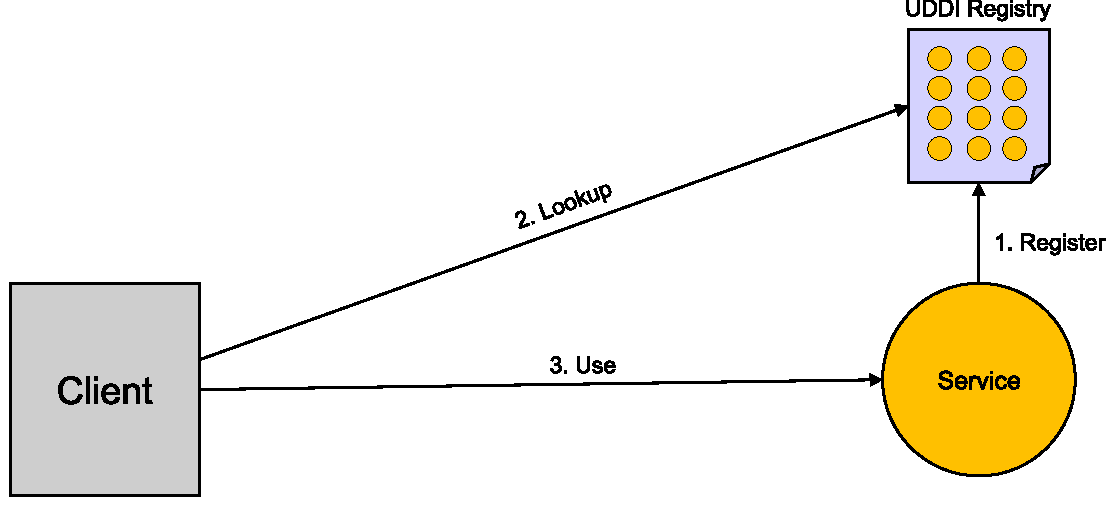
\includegraphics[width=100mm]{09/images/uddi-concept}
\end{figure}
 % AOS
    %!TEX root=../oi-magistr-si.tex
\section[AOS - WS]{Webové služby. K čemu slouží? Popis a vyhledávání služeb. Technologie pro implementaci a nasazení služeb a klientů. Protokoly, kódování obsahu. Top-down a bottom-up design}

\subsection{Webové služby}
W3C definice - SW systém designovaný k vzájemné \textit{machine-to-machine} spolupráci přes internet, který má API přístupné přes \textbf{HTTP}, rozhraní je popsáno v strojové čitelném formátu (\textbf{WSDL}) a interakce s WS je pomocí \textbf{SOAP}  zpráv (HTTP + XML).

\paragraph{RPC Web Service} RPC webové služby představují volání vzdálené funkce. Metoda je popsána jako operace ve WSDL. Parametry metody i odpověď jsou posílány jako XML zabalené v SOAP. Vetšinou je implementováno jako mapování služby přímo na jazykově specifické volání funkce. Není tedy loosely coupled.

\paragraph{SOA Web Service} Webové služby se také používají k implementaci SOA, kde je základní jednotkou komunikace zpráva, nikoli operace. Tato skutečnost je často označována jako „message-oriented“ služba.
Na rozdíl od RPC webových služeb jsou SOA webové služby loose coupled, jelikož jsou zaměřeny na kontrakt poskytnutý WSDL, ne na implementační detaily.

\paragraph{RESTfull Web services} RESTfull webové služby jsou speciální podmnožinou webových služeb, které mají sadu předem definovaných operací. Tyto předem definované operace jsou přímo operace převzaté z protokolu HTTP, jedná se tedy o operace GET, POST, HEAD, atd. Každá z operací má vymezené svoje postavení vůči zdroji, který je identifikován pomocí URL. Následující tabulka shrnuje použití jednotlivých HTTP funkcí z pohledu REST služeb.

Využití metod ve správném významu je zcela klíčové pro čisté REST služby. Existuje mnoho reálných implementací webových služeb, kde je právě tento princip porušen.


\subsection{Vyhledávání služeb - UDDI registr}
UDDI (The Universal Description, Discovery and Integration Service) poskytuje mechanismus, přes který mohou klienti dynamicky hledat požadované webové služby. Tímto způsobem by aplikace měly být schopny se kontaktovat na služby poskytované externími partnery. Registr UDDI má dva druhy klientů: ty, kteří chtějí nějakou službu poskytovat a ty, kteří chtějí službu využívat.

\begin{itemize}[itemsep=0px]
\item platformně nezávislý XML-based registr služeb
\item mechanismus pro hledání WS
\item registry:
\begin{itemize}[itemsep=0px]
\item white pages - adresy, kontakty, identifikátory
\item yellow pages - kategorizace servis založena na standartních taxonomiích
\item green pages - technický popis servis (jak k ní přistoupit atd.)
\end{itemize}
\end{itemize}

\begin{figure}[h!]
\centering
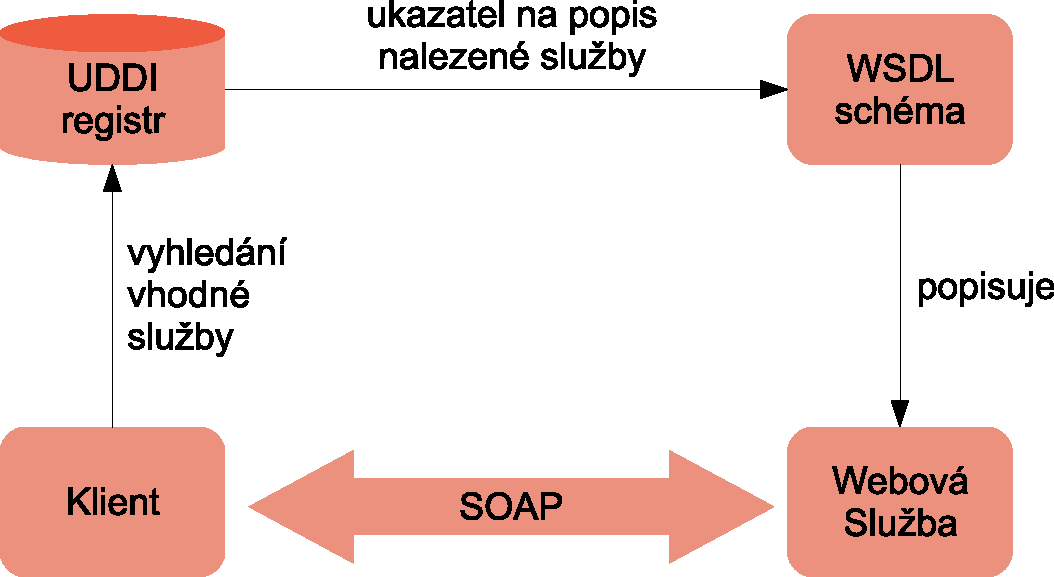
\includegraphics[width=100mm]{10/images/uddi}
\end{figure}

\subsection{Technologie a protokoly}
\subsubsection*{RPC (Remote Procedure Call)}
\begin{itemize}[itemsep=0px]
\item technologie dovolující programu vykonat proceduru (zavolat službu), která může být uložena na jiném místě než je umístěn sám volající program
\item klient/server model
\item synchronní volání klienta - je blokován dokud server neodpoví
\item může nastat chyba v případě chyby sítě
\end{itemize}

\paragraph{Postup} Nejprve proběhne jednoduché zabalení parametrů a identifikátorů procedury do formy vhodné pro přenos mezi počítači (tzv. \textit{marshalling} (serializace)). Poté se balíček odešle. Balíček se na vzdáleném místě rozbalí, zjistí se o jakou proceduru jde (\textit{unmarshalling}). Následuje samotné zavolání a provedení procedury. Výsledek procedury se opět zabalí a odešle zpět. První počítač výsledek opětovně rozbalí. A přijatá hodnota se předá proceduře.

\subsubsection*{CORBA (Common Object Request Broker Architecture)}
\begin{itemize}[itemsep=0px]
\item standard, který umožňuje komunikaci mezi různými platformami a jazyky
\item \hl{jazykově, technologicky a platformě nezávislý}
\item specifikace zahrnuje: silné typování, výjimky, síťový protokol
\item CORBA IDL (Interface Definition Language)
\item transakce, security, marshalling
\end{itemize}

\hl{Je to objektová sběrnice, která objektům umožňuje transparentně vysílat požadavky (requests) směrem k jiným objektům (ať již lokálním nebo vzdáleným) a následně od těchto objektů přijímat odpovědi (replies).} Toto prostředí je nezávislé jak na programovacím jazyce, tak na operačním systému či hardwarové  platformě.

Pro komunikaci mezi CORBA objekty jsou důležité specifikace jejich rozhraní v  jazyce IDL (Interface Definition Language). Ty slouží jako jakási forma kontraktu mezi CORBA objekty a jejich potenciálními klienty jinak řečeno, \hl{klient volá pouze metody nad rozhraním definovaným v IDL, a nestará se o to, jakým způsobem je daný objekt implementován.} IDL specifikace rozhraní jsou následně, s pomocí IDL kompilátoru, mapovány do konkrétních programovacích jazyků, ve kterých jsou již pak dané CORBA objekty implementovány. Použitím tohoto mechanismu dochází k oddělení implementace CORBA objektů od jejich rozhraní, čímž se dosahuje již jednou zmíněné nezávislosti CORBA prostředí na programovacím jazyce.

\paragraph{Volání metod CORBA objektů}
\hl{Vzdálený CORBA objekt} je v klientském adresovém prostoru \hl{zastupován jiným objektem, tzv. \textit{proxy}}. Proxy má obvykle stejné rozhraní jako cílový objekt, a jeho metodami jsou tzv. \hl{\textit{stuby}} (stubs). Stubem se označuje kód, který vezme všechny parametry volání, vloží je spolu s identifikací dané operace do zprávy (marshalling) a tuto zprávu předá jádru ORBu k doručení směrem k cílovému objektu. Na straně serveru předá ORB došlou zprávu skeletonu. Úkolem skeletonu je vyjmout z ní identifikaci požadované operace spolu s jejími parametry, a tuto 
operaci zavolat nad implementací CORBA objektu. Formát zpráv předávaných mezi klientem a serverem je specifikován protokolem  IIOP (Internet Inter-ORB Protocol), který zajišťuje interoperabilitu mezi ORBy různých výrobců.
Z popsaného mechanismu je patrno, že lokální volání metody nad proxy má tedy za následek pro klienta transparentní vyvolání odpovídající metody nad vzdáleným objektem (tento mechanismus již známe z RPC). Poznamenejme pouze, že kód klientského proxy i serverovského skeletonu je automaticky generován IDL kompilátorem na základě popisu rozhraní cílového CORBA objektu \cite{corba}.

\begin{figure}[h!]
\centering
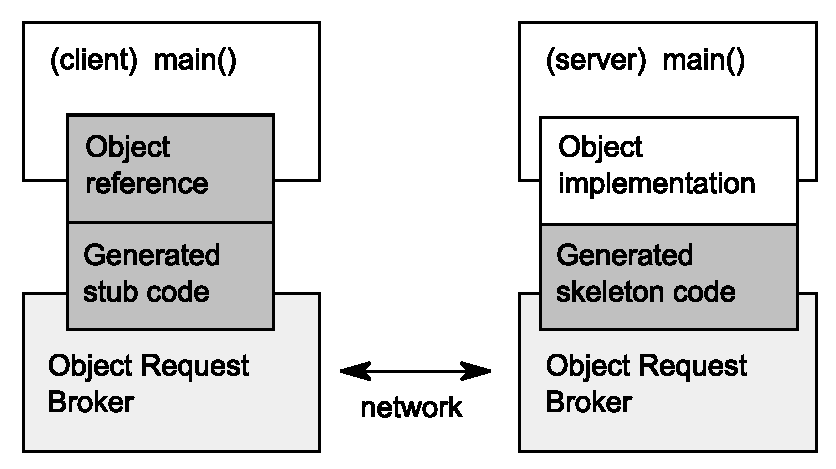
\includegraphics[width=80mm]{10/images/corba}
\caption{CORBA}
\end{figure}

\subsubsection*{DCOM (Distributed Component Object Model)}
\begin{itemize}[itemsep=0px]
\item \hl{microsoftí CORBA} (konkurent)
\item garbage collecting - uvolnění referencí držených klientem (např. při ztrátě spojení)
\end{itemize}
\subsubsection*{WSDL (Web Services Description Language)}
\begin{itemize}[itemsep=0px]
\item \hl{XML-based jazyk, který poskytuje popis (rozhraní) služby}
\item služby jsou definovány jako množina síťových endpointů (portů s adresami a bindováním)
\item popisuje veřejný interface služby
\end{itemize}
\subsubsection*{REST (Representational State Transfer)}
\begin{itemize}[itemsep=0px]
\item architektonický styl nebo množina principů pro tvorbu WS
\item klienti/servery
\item klient se dotáže - server zpracuje požadavek a vrátí odezvu
\item původně popsán pro HTTP (ale není na něj omezen)
\item vlastnosti:
\begin{itemize}[itemsep=0px]
\item stateless
\item cacheable
\item layered system
\item code on demand (opt)
\item uniform interface
\end{itemize}
\end{itemize}
\subsubsection*{SOAP (Simple Object Access Protokol)}
Jelikož veškerá komunikace mezi službami je založená na posílání zpráv, musely být zavedeny takové standardy, aby služby mezi sebou komunikovaly jednotným způsobem. Takovýmto standardem se stal SOAP. SOAP je protokol umožňující spotřebiteli služeb komunikovat s jejich poskytovatelem. Tento protokol je nezávislý na typu sítě, podporuje zprávy ve formátu XML a v současné době je ve specifikaci 1.2 od organizace W3C.

\begin{itemize}[itemsep=0px]
\item specifikace pro výměnu strukturovaných informací pomocí webových služeb
\item SOAP je nezávislý na transportních protokolech. HTTP je jen jedním z podporovaných.
\item postaveno na WSDL a UDDI
\item navrženo jako object-access protokol
\end{itemize}

\begin{wrapfigure}{r}{0.35\textwidth}
  \begin{center}
    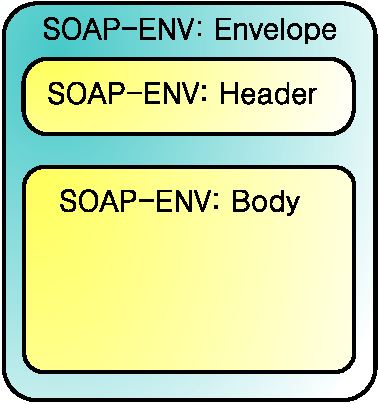
\includegraphics[width=0.28\textwidth]{10/images/soap-message}
  \end{center}
  \vspace{-10px}
  \caption{SOAP zpráva}
\end{wrapfigure}

\paragraph{Struktura zprávy v SOAP}
Každá zpráva dodržující podmínky kladené SOAP je v podstatě balíček (obálka, angl. envelope). Tento balíček obsahuje hlavičku (angl. head) a tělo (angl. body). Hlavička se skládá z několika bloků, které obsahují metainformace. Hlavička je nepovinná (tzn. může být vynechána). Metainformace v sobě ukrývají část komunikační logiky a obecně umožňují zavádět nová rozšíření. Typicky hlavička obsahuje nutné informace pro všechny služby, které mohou zprávu obdržet. Cílová služba potom na základě těchto informací rozhodne o způsobu zpracování zprávy. Tělo obsahuje samotná data (ve formátu XML). Tělo může také obsahovat sekci pro
chyby (angl. faults), která obsahuje logiku pro zpracování výjimek. Většinou jsou v této části uloženy jednoduché zprávy, které slouží k odeslání informací o chybě při výskytu výjimky. SOAP zahrnuje také prostředky pro posílání dat, která jsou těžko popsatelná pomocí XML (binární data, např. obrázky). Takováto data se posílají jako přílohy (angl. attachments).

\subsection{Kódování obsahu}
\hl{Posílaný obsah} je potřeba nějakým způsobem reprezentovat. Požadavky jsou aby \hl{\textbf{reprezentace}} (zakódování) byla lidsky \hl{\textbf{čitelná}, \textbf{neukecaná}} (binary efficient - chceme posílat co nejmenší obsah), platformně \textbf{nezávislá} a \textbf{standardizovaná}.

\begin{itemize}[itemsep=0px]
\item XML - příliš ukecané
\item \hl{JSON - používané}
\item YAML
\item buffers by Google
\end{itemize}

\subsection{Bottom-up design}
Nejdříve je naimplementována služba v konkrétním jazyce, následně je vygenerováno WSDL. Považováno za jednodušší návrh. Riziko vzniku závislosti na programovacím jazyku či platformě.

\subsection{Top-down design}
Nejdřive je napsán WSDL dokument (koresponduje s SOA modelem), následně je z něj vygenerován kód. Považováno za obtížnější. výsledkem je ale čistší design.
 % AOS
    %!TEX root=../oi-magistr-si.tex
\section[AOS - Kompozice služeb]{Webové služby, automatická kompozice služeb. Orchestrace a choreografie, web mash-up. Modelování služeb a procesů (BPMN, BPEL).}

Na kompozitní službu se můžeme dívat jako na sadu služeb, které spolu spolupracují za účelem vykonání určitého procesu, který definuje interakční workflow. \textbf{Orchestrace} a \textbf{choreografie} jsou rozdílné vzory pro vytváření kompozice služeb. Jazyky pro popis vykonávaného procesu (a tedy i pro popis spolupráce služeb) jsou např. BPMN, BPEL, UML.

\subsection{Orchestrace}
Při tomto přístupu je centrální prvek, který koordinuje všechny zapojené služby. Tento centrální prvek může být také webová služba. Zúčastněné služby nevědí, a ani nemusí vědět, že jsou účastníky nějakého většího procesu, o tom ví jen centrální prvek. Iterakce při orchestraci nastávají na úrovni zpráv.

\subsection{Choreografie}
U choreografie není centrální prvek procesu, a proto všechny zapojené služby ví, kdy volat a s kým dalším spolupracovat.

V praxi se více využívá orchestrace, protože se díky centrálnímu prvku lépe zotavuje z chyb (chyby jsou odchytávány na jednom místě).

\subsection{Mashup}
Aplikace kombinující data/funkcionalitu z 2 a více zdrojů.

\begin{itemize}[itemsep=0px]
\item Client-based - všechny data se z více služeb volají z klientova prohlížeče (problém s javascriptem Same-Origin Security Policy - POST dotazy).
\item Server-based - Prostředník v podobě serveru, uživatel se dotazuje na jeden server, a ten za něj získává data z ostatních služeb.
\end{itemize}

\subsection{Modelovací jazyky BPMN, BPEL}

\paragraph{BPMN (Business process modeling notation)} Grafická reprezentace pro specifikaci byznys procesu. Podobné UML. Poskytuje mapování mezi grafickou notací a BPEL.

\begin{figure}[h!]
\centering
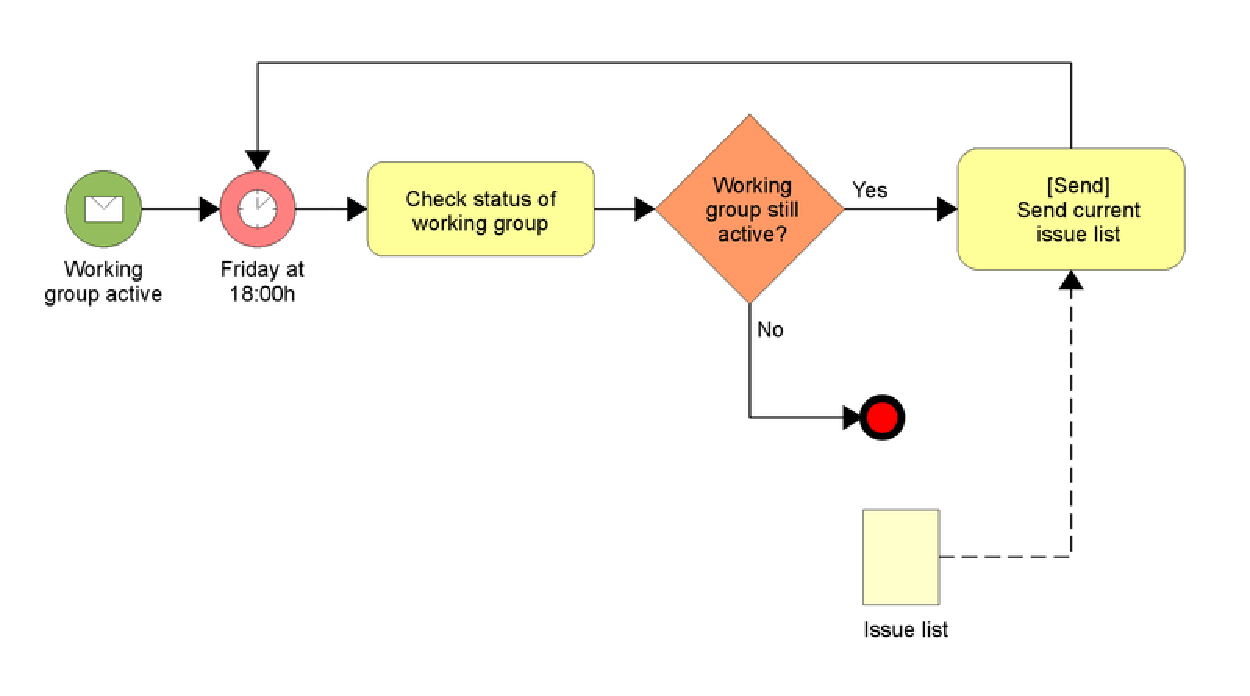
\includegraphics[width=100mm]{11/images/bpmn}
\end{figure}

\paragraph{BPEL} Business Process Execution Language je jazyk pro popis WS kompozice. Základ toho jazyka tvoří WSFL a XLANG. WSFL je zkratka pro Web Services Flow Language, jazyk vytvořený IBM pro popis kompozice webových služeb. XLANG je rozšíření WSDL. Zjednodušeně se dá říct, že popis služby v XLANG se skládá z popisu dané služby ve WSDL a popisu chování služby jako části byznys procesu. Varianta BPEL pro webové služby se označuje BPEL4WS (někdy také WS-BPEL). Tento jazyk rozšiřuje základní interakční schéma mezi službami o podporu byznys transakcí.

Je to programovací jazyk v XML?

BPMN --> BPEL --> Application % AOS
    %!TEX root=../oi-magistr-si.tex
\section[AOS - Kvalita, bezpečnost]{Architektura zaměřená na služby (SOA). Kvalita, výkonnost a škálování služeb. Zabezpečení, integrita, bezpečnost, a autentifikace služeb. Point-to-point a end-to-end šifrování.}

\url{http://www.w3c.or.kr/kr-office/TR/2003/ws-qos/}

\paragraph{Výkonnost}
Výkonnost reprezentuje jak rychle služba zpracuje dotaz. To může být měřeno dobou odezvy, dobou spouštění, nebo doby jednotlivých transakcí.

\paragraph{Spolehlivost}
Schopnost poskytnout službu na požádání uživatelem a poskytovat ji po požadovanou dobu v rámci specifikovaných tolerancí a dalších daných podmínek.

\paragraph{Škálovatelnost}
Schopnost zvyšování výpočetní kapacity za účelem zvýšení výkonnosti a kapacity. Služba by měla být škálovatelná ve smyslu navýšení počtu operací a transakcí.

\paragraph{Kapacita}
Služba by měla být poskytována s požadovanou kapacitou, tzn. garantovaným výkonem při zadaném počtu (kapacitě) paralelních requestů.

\paragraph{Robustnost}
Robustnost značí schopnost správného fungovaní služby i při nevalidních (nekompetních, konfliktních) vstupech.

\paragraph{Zpracování výjimek}
Služby by měli být poskytovány s funkcionalitou zpracování chyb a výjimek.

\paragraph{Integrita}
Služba umí předcházet/bránit neopravněnému přistupu nebo modifikaci k datům. Jsou dva typy integrity: datová a transakční.

\paragraph{Přístupnost}
Přistupnost je schopnost obsluhovat klientské požadavky (requesty). Dostupnost se dá navýšit vytvářením škálovatelných služeb.

\paragraph{Dostupnost}
Chceme co nejvyšší dostupnost služby, jako parametr se udává Time-to-Repair (TTR).

\paragraph{Bezpečnost}
Service Security Performance - Odolnost proti neoprávněnému odposlechu, neoprávněnému použití, zlovolnému poškození, nesprávnému použití, lidským chybám a přírodním katastrofám.

\subsection{Bezpečnost}
Poskytuje se bezpečnost klienta, serveru a zpráv. Bezpečnost zpráv je pokryta kryptografií (symetrické/asymetrické šifrování, digitální podpisy a certifikáty). U bezpečnosti klienta je řešeno: service discovery risk, phishing risk, autenticita a korektnost přijatých zpráv, autentikace poskytovatelů služeb.


\paragraph{Point-to-point}
Communication channel level. Guarantied on the server basis
\begin{figure}[h!]
\centering
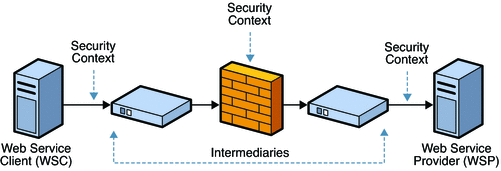
\includegraphics[width=80mm]{12/images/security-p2p}
\end{figure}

\paragraph{End-to-end}
Message level. Application oriented security

\begin{figure}[h!]
\centering
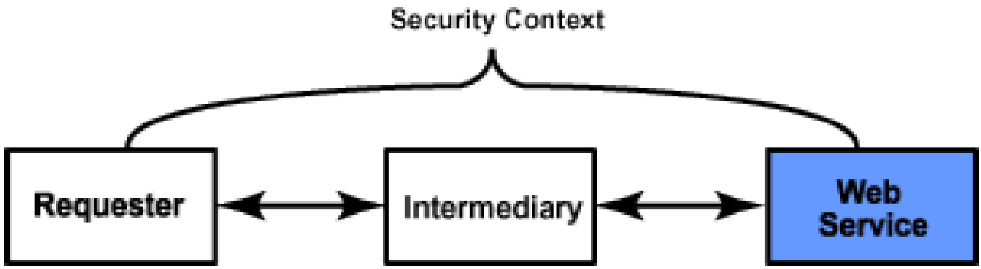
\includegraphics[width=80mm]{12/images/security-e2e}
\end{figure}

\begin{itemize}[itemsep=0px]
\item \textbf{XML signatura} - Podepisuje se buď celý dokument, nebo jen část
\item \textbf{XML šifrování} - end-to-end, v soap obálce je oddíl se security tokenem a signaturou.
\end{itemize}
 % AOS
    %!TEX root=../oi-magistr-si.tex
\section[TVS - Chyby,optimalizace testů,test. automatů]{Kategorizace SW chyb, optimalizace návrhu testů. Testování automatů.}

SW chyba je prezentace toho, že program dělá něco nepředpokládaného. Je to míra toho, kdy program přestává být užitečný (lidem). Je to nesouhlas mezi programem a jeho specifikací (pouze tehdy, jestliže specifikace existují a jsou správné!).

\begin{figure}[h!]
\centering
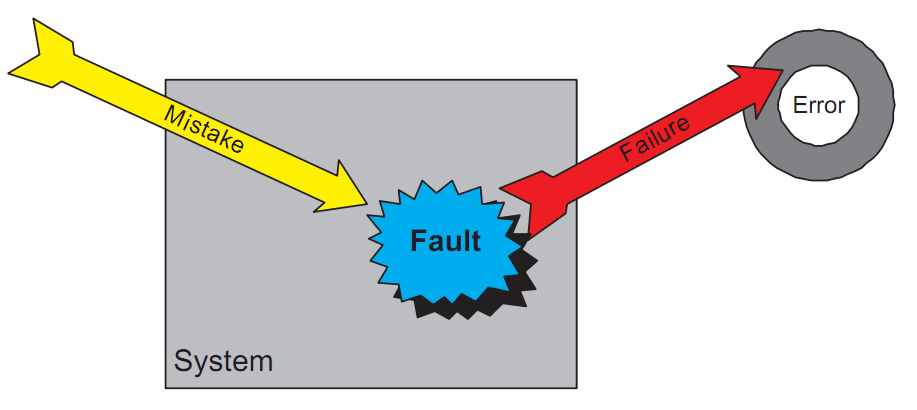
\includegraphics[width=80mm]{13/images/chyba}
\end{figure}

\begin{itemize}[itemsep=0px]
\item \textbf{Pochybení}: Akce člověka, která produkuje nesprávný výsledek.
\item \textbf{Vada}: Nesprávný krok, proces nebo definice dat v počítačovém programu. Výsledek pochybení. Potenciálně vede k selhání.
\item \textbf{Selhání}: Nesprávný výsledek. Projev vady.
\item \textbf{Chyba}: Kvantitativní vyjádření toho, na kolik je výsledek nesprávný
\end{itemize}

\subsection{Kategorie SW chyb}

\begin{itemize}[itemsep=0px]
\item \hl{Chyby UI} - vstupy (nápověda), výstupy (rychlost odezvy)
\item \hl{Chyby omezení} - výjimky, výpočetní chyby
\item \hl{Procesní chyby} - chyba při první inicializaci, zátěž, souběh více vláken
\item \hl{Chyby vedení} - stará verze knihovny, slabá doc
\item \hl{Chyby požadavků, vlastností a funkčnosti} - neúplné, nejednoznačné
\item \hl{Strukturální chyby} - logika (neporozumění log. operátorům), GOTO, konverze typů
\item \hl{Datové chyby} - specifikace objektů
\item \hl{Chyby implementace} - syntaktické chyby, chyby paměti, hranice pole
\end{itemize}
\paragraph{Chyby uživatelského rozhraní}
\begin{itemize}[itemsep=0px]
\item Problémy s funkčností - program nedělá něco, co by měl dělat nebo to dělá nevhodně (zmatečně, neúspěšně), lze některé operace provést obtížně.
\item To co se \uv{předpokládá} od programu, žije pouze v mysli uživatele
\item Všechny programy mají problémy s funkčností vzhledem k různým uživatelům.
\item Funkční problém je chybou, pokud očekávání uživatele jsou rozumná.
\item \textbf{Vstupy}

    \begin{itemize}[itemsep=0px]
    \item Jak lze nalézt, jak program používat (jaká je nápověda)?
    \item Jak snadné je ztratit se v programu?
    \item Jaké chyby uživatel dělá a kolik ho to stojí času?
    \item Co mu chybí?
    \item Nutí prg. uživatele přemýšlet nepřirozeně?
    \end{itemize}
    
\item \textbf{Výstupy}

    \begin{itemize}[itemsep=0px]
    \item Rychlost je základ interaktivního sw.
    \item Cokoli co budí dojem pomalého prg. je problém.
    \item Získá uživatel, co potřebuje?
    \item Mají výstupy smysl?
    \item Může uživatel přizpůsobit výstup potřebám?
    \item Zle výstup přesměrovat dle potřeby(monitor, tisk, soubor, $\hdots$)?
    \end{itemize}
\end{itemize}
\paragraph{Chyby omezení}

\begin{itemize}[itemsep=0px]
\item Chyby zpracování vyjímek zahrnující neschopnost
    \begin{itemize}[itemsep=0px]
    \item Předvídání možnosti chyby a bránit se jim
    \item Zpracování podmínek chyby
    \item Zpracovaní detekované chyby různými způspby
    \end{itemize}
\item Chyby hraničních podmínek
    \begin{itemize}[itemsep=0px]
    \item Nejjednodušší hranice jsou numerické
    \item Mezní nároky na paměť, za kterých program může pracovat
    \end{itemize}
\item Výpočetní chyby
    \begin{itemize}[itemsep=0px]
    \item Chyby aritmetiky jsou časté a obtížně detekovatelné
    \item Program ztrácí přesnost během výpočtu vlivem zaokrouhlovacích chyb a ořezání
    \item Výpočetní chyby způsobené chybnými algoritmy
    \end{itemize}
\end{itemize}

\paragraph{Procesní chyby}
\begin{itemize}[itemsep=0px]
\item Sekvenční
    \begin{itemize}[itemsep=0px]
    \item Počáteční a jiné speciální stavy
        \begin{itemize}[itemsep=0px]
        \item Funkce mohou selhat při prvním použití, např. chybějící inicializační informace či soubory
        \item Nastaví se skutečně vše do výchozího bodu, vymažou se všechna data, jestliže uživatel provede reset programu?
        \end{itemize}
    \item Chyby řízení nastane, pokud program provede chybný příští krok
        \begin{itemize}[itemsep=0px]
        \item Extrémní chyba nastane, pokud se program zastaví nebo vymkne kontrole řízení
        \end{itemize}
    \end{itemize}
\item Paralelní
    \begin{itemize}[itemsep=0px]
    \item Chyby souběhu - race error
        \begin{itemize}[itemsep=0px]
        \item Jedny z nejméně testovaných
        \item Nastávají v multiprocesových sys. a integračních sys.
        \item Velmi obtížně se opakují
        \end{itemize}
    \item Zátěžové podmínky
        \begin{itemize}[itemsep=0px]
        \item Program se začne chovat chybně pokud se přetíží
            \begin{itemize}[itemsep=0px]
            \item Chyby velkého objemu - hodně práce za dlouhou dobu
            \item Chyby velkého stresu - hodně práce v daném okamžiku
            \end{itemize}
        \item Všechny programy mají své limity, ale je důležité vědět co nastane
        \end{itemize}
    \end{itemize}
\end{itemize}

\paragraph{Chyby vedení}
\begin{itemize}[itemsep=0px]
\item Hardware - program posílá chybová data na zařízení, ignorují chybové kódy přicházející zpět a zkouší použít zařízení, která neexistují nebo jsou aktuálně vytížená
\item Řízení zdrojů a vedení
    \begin{itemize}[itemsep=0px]
    \item Staré problémy se opět objevují, pokud programátor zakomponuje do programu nějakou starou verzi komponenty
    \item Ujistěte se, že program má správný copyright, vstupní obrazovky a
    \end{itemize}čísla verzí
\item Dokumentace - slabá dokumentace může způsobit ztrátu víry uživatele, že sw. pracuje spráně
\item Chyby testování
    \begin{itemize}[itemsep=0px]
    \item Chyby udělané testy jsou nejčastějšími chybami objevenými během testování
    \item Jestliže program navádí většinu uživatelů ke způsobení chyb, pak je špatně navržen
    \end{itemize}
\end{itemize}
    
\paragraph{Chyby požadavků, vlastností a funkčnosti}

\begin{itemize}[itemsep=0px]
\item Požadavky a specifikace
    \begin{itemize}[itemsep=0px]
    \item Neúplné, nejednoznačné, vzájemně si odporující
    \item Hlavní zdroj drahých chyb
    \end{itemize}
\item Chyby vlastností - chybějící, chybné, nevyžádané vlastnosti
\item Interakce vlastností - nepredikované interakce(přesměrování telefonu ve smyčce)
\item Preventivní opatření proti chybám ve specifikacích a vlastnostech:
    \begin{itemize}[itemsep=0px]
    \item Problém v komunikaci člověk-člověk
    \item Jazyk formálních specifikací poskytující krátkodobé řešení, avšak neřeší problém chyb v dlouhodobém horizontu.
    \end{itemize}
\end{itemize}
    
\paragraph{Strukturální chyby}
\begin{itemize}[itemsep=0px]
\item Chyby v řízení sekvencí
    \begin{itemize}[itemsep=0px]
    \item Příkaz GOTO
    \item Většina chyb řízení (v novém kódu) se dá snadno testovat a je chycena během testování jednotek
    \item Neupravený starý kód může mít řadu chyb v řídicím toku
    \item Stlačování za účelem kratšího prováděcího času nebo menšího nároku na paměť je špatná politika
    \end{itemize}    
\item Chyby zpracování
    \begin{itemize}[itemsep=0px]
    \item Zahrnuje chyby vyhodnocení aritmetických, algebraických nebo matematických fcí. a výběr algoritmu
    \item Řada problému vznikne špatnou konverzí dat na jinou reprezentaci
    \end{itemize}
\item Chyby logiky
    \begin{itemize}[itemsep=0px]
    \item Neporozumění jak se selekční či logické operátory chovají samostatně nebo v kombinacích
    \item Neporozumění sémantice uspořádání logických výrazů a jeho vyhodnocení specifickými překladači
    \item Chyby datového toku - nevztahují se k chybám řízení
    \item Chyby toku řízení - část logického výrazu, která je použita pro ovládání toku řízení
    \end{itemize}
\item Inicializační chyby - opomenutí inicializace pracovního prostoru, registů, nebo části dat
\item Chyby a anomálie toku dat
    \begin{itemize}[itemsep=0px]
    \item Nastane pokud existuje cesta, při které se udělá s daty něco neodůvodněného např. použití neinicializované proměnné, nebo neexistující proměné
    \item Jsou stejně tak důležité jako anomálie toku řízení
    \end{itemize}
\end{itemize}
    
\paragraph{Datové chyby}
\begin{itemize}[itemsep=0px]
\item Lze je nalézt ve specifikacích datových objektů, jejich formátů, počtu nebo jejich počátečních hodnotách
\item Sw. se vyvíjí k tabulkám obsahujících řídicí a procesní fce.
\item Trendy programování vedou k zvýšenému používání nedeklarovaných, interních, speciálních programovacích jazyků
\item Dynamické vs. statické
    \begin{itemize}[itemsep=0px]
    \item Protože efekt poškození dynamických dat se může projevit velmi vzdáleně od příčiny, nalézají se takovéto chyby velmi obtížně
    \item Základní problém zbytků ve sdílených zdrojích (např. vyčištění po použití uživatelem, sdílené čištění pomocí ovladače zdrojů, žádné čištění)
    \end{itemize}
\item Informace, parametr, řízení
    \begin{itemize}[itemsep=0px]
    \item Údaj plní jednu ze tří rolí: jako parametr, jako řízení, jako zdroj informace
    \item Informace je obvykle dynamická s tendencí lokality pro danou transakci (nedostatek ochranného kódu validace dat)
    \item Neadekvátní validace dat často vede k ukazování prstem
    \end{itemize}
\item Obsah, struktura, atributy
    \begin{itemize}[itemsep=0px]
    \item Obsah - aktuální bitový vzor, řetězec znaků, nebo číslo vložené do datové struktury
    \item Struktura - velikost, tvar a počty popisující datové položky
    \item Atributy - specifikace významu (sémantika)
    \item Základem je explicitní dokumentace obsahu, struktury a atributů všech datových objektů
    \end{itemize}
\end{itemize}

\paragraph{Chyby implementace}
\begin{itemize}[itemsep=0px]
\item Chyby kódování
    \begin{itemize}[itemsep=0px]
    \item Dobrý překladač chytne syntaktické chyby, nedeklarovaná data, procedury, kód a mnoho inicializačních problémů
    \item Častou chybou kódu jsou dokumentační chyby (komentáře)
    \item Úsilí programování je dominováno údržbou
    \end{itemize}
\item Chyby paměti
    \begin{itemize}[itemsep=0px]
    \item Charakteristiky
        \begin{itemize}[itemsep=0px]
        \item Nejobtížnější chyby z hlediska lokalizace
        \item Nejdůležitější chyby z hlediska opravy
        \item Projevy nesprávného obsahu paměti jsou nepredikovatelné
        \item Chyby v obsahu paměti se typicky projevují vzdáleně od jejich příčiny
        \item Chyby zůstávají často nedetekováné dokud nejsou náhodně spuštěny
        \end{itemize}
    \item Typy chyb
        \begin{itemize}[itemsep=0px]
        \item Chyby hranic polí
        \item Přístup přes nedefinovaný ukazatel
        \item Čtení z neinicializované paměti
        \item Chyby ztráty paměti (memory leaks)
        \end{itemize}
    \item Slabá místa výkonnosti
        \begin{itemize}[itemsep=0px]
        \item Kolekce vyčerpávající přesné množiny dat pro výkonnostní test programu a každé jeho komponenty (profilování)
        \item Zaměření se na kritická data
        \item Sběr správně vybraných dat
            \begin{itemize}[itemsep=0px]
            \item Řádka - kolikrát proběhla každá řádka - nejpřesnější, ale nejnáročnější na sběr dat
            \item Funkce - méně podrobné než předchozí
            \item Čas - data se sbírají z údajů časovaných běhů funkcí. Data jsou správná pro daný běh, ale závisí na stavu mikroprocesoru a paměti. Nejméně náročný sběr
            \end{itemize}
        \end{itemize}
    \end{itemize}
\end{itemize}

\subsection{Optimalizace návrhů testů}

Optimalizovat testování chceme za účelem snížení jeho časové náročnosti. Např. u PLC chceme testovat instrukci, která má 5 parametrů a každý z nich může nabývat 17ti hodnot. To je $17^5$ kombinací (1 419 857) tedy cca 230 dnů testování.

V praxi se ale ukázalo, že většina chyb nevzniká při všech 5ti nastavených parametrech, ale při interakci jen několika z nich. Vytvářejí se pak testy, které pokrývají jen všechny možné k-tice (ne všechny kombinace). Pomocí následujících metod se dá počet testovaných případů redukovat.

\subsubsection{Princip párového testování}
Jak již bylo zmíněno, při \textbf{ideálním testovacím plánu} by bylo nutné projít všechny kombinace hodnot parametrů, tj. $1 419 857 = 17^5$ kombinací - 230 dnů testování.


Praktický testovací plán využívá toho, že selhání jsou způsobena interakcí pouze několika parametrů, Proto se provádí testování kombinacemi pokrývající všechny možné k-tice (k-tice komprimovány do plných kombinací).

\paragraph{Příklad}
\begin{itemize}[itemsep=0px]
\item 5 parametrů
\item 17 hodnot pro každý parametr
\item \textbf{Optimalizace:}
\item Nezávislé parametry: 17 kombinací,
\item Počet párů: 5 nad 2 = 10 parametrových párů,
\item Hodnot pro každý pár: $289 = 17^2$ kombinací hodnot pro každý pár,
\item Počet hodnot pro všechny pár: $2890 = 289*10$ párů parametrových hodnot,
\item zredukovaných 289 kombinací obsahující všechny páry,
\item 30 minut testování.
\end{itemize}

\subsubsection{Optimalizace metodou ortogonálních polí}
Ortogonální pole je matice velikosti $m \times n$, ve které při testování parametrických párů jednotlivé sloupce odpovídají faktorům (parametrům funkce, případně jiným hodnotám, na kterých závisí testovací případ) a řádky jednotlivým testovacím případům.

Ortogonální pole jsou označována podle toho, kolik úrovní (významných hodnot) umožňují jednotlivým faktorům. Ortogonální pole $(2^{1} \times 3^{7})$ má celkem 8 faktorů. Jeden faktor může mít dvě významné hodnoty, a sedm dalších může mít až 3 významné hodnoty.

Pro použití této techniky je zapotřebí příklad nejprve zakódovat. Tato procedura je velmi snadná – nejprve nalezneme všechny faktory (parametry příkladu) a zjistíme, kolik mají úrovní. Poté nalezneme vhodné ortogonální pole.

Vybrané pole musí umožňovat alespoň tolik faktorů, kolik má náš případ. Dále je nutné, aby jednotlivé faktory měly dostatečný počet úrovní.

Nyní můžeme přejít k samotnému kódování. Každému parametru naší úlohy přiřadíme jeden sloupec – případné přebytečné sloupce můžeme ignorovat. Každé významné hodnotě přiřadíme jednu úroveň – pokud má sloupec více úrovní než potřebujeme, tak můžeme některé významné hodnotě přiřadit více úrovní, tím tuto hodnotu otestujeme více než ostatní (ale stále platí, že otestujeme každou parametrickou dvojici alespoň jednou).

V tomto okamžiku již můžeme pomocí našeho zakódování číst jednotlivé řádky ortogonálního pole - samotné testovací případy.

Ortogonální pole není jednoduché nalézt, testovací případy musí být balancované atd., proto existují jejich katalogy (pole nekonstruujeme, ale používáme již dostupná pole z katalogů).

\begin{table}[h]
\begin{tabular}{|l|l|l|l|}
\hline
  & 1 & 2 & 3 \\ \hline
1 & 1 & 1 & 1 \\ \hline
2 & 1 & 2 & 2 \\ \hline
3 & 2 & 1 & 2  \\ \hline
4 & 2 & 2 & 1 \\ \hline
\end{tabular}
\vspace{10px}
\caption{Ortogonální pole $L_4 (2^3)$}
\end{table}

\subsubsection{Optimalizace metodou latinských čtverců}


\textbf{Latinský čtverec} je matice s $n$ řádky a $n$ sloupci taková, že každý element obsahuje celé číslo do 1 do $n$ tak, že se v žádném sloupci nebo řádku nevyskytuje žádné číslo vícekrát než jednou.

\textbf{Párově ortogonální latinské čtverce} - každý elment v daném čtverci vystupuje v relaci s každým elementem druhého čtverce právě jedenkrát. Pro jakoukoliv mocninu prvočísla $n$ existuje $n-1$ párově ortogonálních latinských čtverců velikosti $n \times n$.

\begin{itemize}[itemsep=0px]
\item ze zadání se identifikují faktory a úrovně
\item určím počet párově-ortogonálních čtverců jako $N$ = max(faktorů-2, nejvyšší\_úroveň)
\item najdu si čtverce v literatuře, ($N+1$) rozměrné
\item nyní generuji testovací případy: první faktor je číslo řádku, druhý faktor číslo sloupce, další hodnoty podle čísel na souřadnicích v jednotlivých čtvercích
\item vygeneruje mi to $(N+1)^2$ testovacích případů
\end{itemize}

\subsection{Testování automatů}
\hl{Konečný automat je výborný model pro testování aplikací řízených pomocí menu} (ovládání aplikace se provádí pomocí výběru položek z menu).

Vrcholy zobrazují stavy (stav aplikace). Hrany mezi stavy reprezentují vyběr položky menu (a tím přechod do dalšího stavu). Automat by měl být silně souvislý, pokud existují oddělené stavy (izolované), tak tyto stavy zavání chybou, jsou podezřelé (nevede k nim položka v menu).

\vspace{-10px}

\paragraph{Skryté stavy}
Test nelze zahájit, pokud systém není potvrzením způsobem v počátečním stavu. Dát si pozor na skryté stavy. Při testování SW můžeme předpokládat věci, které nemusí obecně platit (např. že víme, ve kterém stavu se systém nachází). Pokud existují skryté stavy tak se typicky nejedna o jeden či dva stavy, ale o celý stavový prostor.

\paragraph{Postup návrhu testů}

\begin{itemize}[itemsep=0px]
\item identifikuj vstupy
\item definuj kódy vstupu
\item idenfikuj stavy
\item definuj kódovaní stavů
\item identifikuj výstupní akce
\item definuj kódování výstupních akcí
\item specifikuj tabulku přechodů a tabulku výstupů - a zkontroluj ji
\item navrhni testy
\item proveď testy
\item pro každý vstup ověř jak přechod tak i výstup
\end{itemize}

Každý test začíná v počátečním stavu. Z počátečního stavu se systém přivede nejkratší cestou k vybranému stavu, provede se zadný přechod a systém se nejkratší možnou cestou přivede opět do počátečního stavu (tzv. okružní cesta).

\paragraph{Formální konstrukce testů}

Nechť $L$ je \textbf{množina vstupních sekvencí} a $q, q'$ dva stavy. $L$ \textbf{rozliší} stav $q$ od $q'$, jestliže existuje sekvence $k$ v $L$ taková, že \textbf{výstup} získaný apikací $k$ na automat ve \textbf{stavu $q$} je \textbf{různý} od \textbf{výstupu} získaný aplikací $k$ na \textbf{stav $q'$}. Chceme minimální automat (tj. takový, který neobsahuje redudantní stavy).

Množina vstupních sekvencí $W$ se nazývá \textbf{charakterizační množina}, jesltiže může rozlišit jakékoliv dva stavy automatu.

\begin{itemize}[itemsep=0px]
\item \textbf{Pokrytí stavů} je množina vstupních sekvencí $L$ taková, že lze nalézt prvek množiny $L$, kterým se lze dostat do jakéhokoliv žádaného stavu z počátečního stavu $q_0$.
\item \textbf{Pokrytí přechodů} minimálního automatu je množina vstupních sekvencí $T$, která je pokrytím stavů a uzavřená z hlediska pravé kompozice s množinou vstupů $Input$.

$$seq \in T = L \bullet (Input \cup {<>})$$

\end{itemize}
 % TVS
    %!TEX root=../oi-magistr-si.tex
\section[TVS]{Testovaní metodami bílé a černé skřínky. Strukturální, statická a dynamická analýza. Analýza datových toků. Testování objektově orientovaného softwaru.}

\subsection{White/black box testování}

Při \textbf{testování černé skříňky} se zaměřujeme na vstupy a výstupy programu bez znalosti, jak je naimplementován. Produkt je černou skříňkou, do které se nelze podívat, vidíme jen jak vypadá a jak se chová navenek. Smyslem je analyzovat chování softwaru vzhledem k očekávaným vlastnostem tak, jak ho vidí uživatel. Do této kategorie spadají skoro všechny druhy \textbf{testů uživatelských rozhraní}, akceptační testy, testování podle scénářů, které krok za krokem provádějí uživatele tím, co má zadat a jaké jsou očekávané reakce systému.

Při \textbf{testování bílé skříňky}, má tester přístup ke zdrojovému kódu a testuje produkt na základě něj. Vidí nejen co se děje na povrchu skříňky, ale i vnitřní reakce systému. Tím poněkud ztrácí pohled uživatele, ale může lépe odhadnout, kde hledat chyby a kde ne. Sem spadají např. \textbf{unit testy}.

\subsection{Strukturální analýza}

Strukturální analýza je převedení programu na model (typicky graf). V grafu se pak dají zobrazit toky řízení, toky dat, stromy závislosti volání funkcí, či grafy konečních automatů

\begin{figure}[h!]
\centering
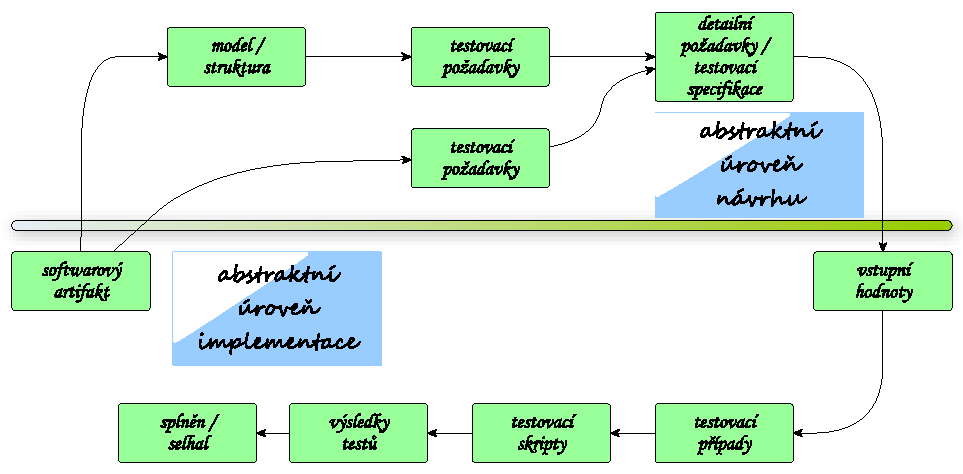
\includegraphics[width=130mm]{14/images/test-model}
\end{figure}

\paragraph{Návrh testování podle modelu}
\begin{itemize}[itemsep=0px]
\item definuj graf, definuj relace
\item navrhni testy pro pokrytí uzlů
\item navrhni testy pro pokrytí hran
\item otestuj všechny atributy
\item navrhni testy smyček
\end{itemize}

\paragraph{Kritéria pokrytí}
\begin{itemize}[itemsep=0px]
\item \textbf{Pokrytí řádek} - požaduje provedení každé řádky kódu alespoň jednou
\item \textbf{Pokrytí větví} - znamená, že podmínka každého větvení musí být alespoň jednou pravdivá a jednou nepravdivá
\item \textbf{Pokrytí podmínek} - zkontroluje všechny možné způsoby, za kterých daná podmínka je pravdivá či nepravdivá
\item \textbf{Úplné pokrytí cest} - vyžaduje provedení všech možných různých úplných cest (v praxi neproveditelné)
\end{itemize}

\subsection{Statická a dynamická analýza}
\textbf{Statická analýza} je model checking (viz následující otázka) a testování konečného automatu.

Analýza kódu, hledájí se v něm logické chyby jako např. nekonečný cyklus, nepoužívané proměnné, přiřazení místo porovnání atd. Řeší to např. pluginy do IDE (nebo IDE samotné).

\textbf{Dynamická analýza} je test běžící aplikace AUT=application under test. Třeba checkování použití paměti (Rational Purify, Boundchecker)

\subsection{Analýza toků řízení (metoda hlavních cest)}

\paragraph{Jednoduchá cesta} Cesta z $n_i$ do $n_j$ na které se žádný uzel neobjevuje více jak jedenkrát s vyjímkou, že počáteční a koncový uzel mohou být identické.

\paragraph{Hlavní cesta} Cesta z $n_i$ do $n_j$ je hlavní, jestliže je to jednoduchá cesta a není žádnou vlastní podcestou jakékoliv jiné jednoduché cesty (tj. je maximální).

\noindent Cílem je nalézt hlavní cesty. \textbf{Princip algoritmu:}

\begin{itemize}[itemsep=0px]
\item Nalezni cesty délky 0 (uzly).
\item Kombinuj cesty délky 0 do cest délky 1 (hrany).
\item Kombinuj cesty délky 1 do cest délky 2.
\item atd.
\end{itemize}

\subsection{Analýza datových toků (metoda du-cest)}
Tok datových hodnot: testy zajišťující, že hodnoty vzniklé na jednom místě jsou použity správně na jiných místech. 

\begin{itemize}[itemsep=0px]
\item \textbf{Definice} \textit{def}: místo, kde je hodnota proměnné uložena do paměti. 
\item \textbf{Užití} \textit{use}: místo, kde se přistupuje k hodnotě proměnné.
\item \textbf{DU páry def-use:} asociace určující přenosy hodnot. 
\end{itemize}

\paragraph{Formalizace}
\begin{itemize}[itemsep=0px]
\item V : množina proměnných asociovaná se softwarovým artefaktem. 
\item def : místo, kde je hodnota proměnné uložena do paměti
\item use : místo, kde se přistupuje k hodnotě proměnné
\item def (n) = podmnožina množiny proměnných $V$, které jsou definovány uzlem $n$
\item use (n) = podmnožina množiny proměnných $V$, které jsou použity v uzlu $n$
\item du(n, v) je množina všech du-cest vzhledem k proměnné $v$, která začíná v uzlu $n$
\end{itemize}

\subsection{Testování OO softwaru}

\paragraph{Anomálie DU párů}

Anomálie souvisí s děděním a polymorfismem.

Jsou třídy A $\leftarrow$ B.

\begin{itemize}[itemsep=0px]
\item \textbf{ITU} - inconsistent type use - nepřepisování ale volání parent metod, nejdřív použiju metody B, pak nějaké z A a pak opět B (A metody mohou něco nečekaně přepsat - přivézt objekt do stavu nekonzistentním s B).

\item \textbf{SDA} - state definition anomaly - přepisící metoda má jinou def množinu než přepisovaná (přepisující metody v B nenadefinují některé proměnné, které jsou definovány přepsanými metodami v A).

\item \textbf{SDIH} - podobné SDA ale potomek přepíše něco v prarodiči a rodič pak používá špatně definovanou proměnnou.

\item \textbf{ACB1} - přepis konstruktoru, potomek pak používá něco co není definováno.

\item \textbf{SVA} - přepsání metody v prarodiči, později rodič taky přepíše tu metodu a potomek začne volat rodiče, ne prarodiče
\end{itemize}

\paragraph{Testování párových sekvencí}

Typy testování: intra/inter metod a intra/inter tříd

Používá se k reprezentace interakce stavových prostorů, identifikace bodů integrace a testovacích požadavků. V softwarových artefaktech se hledají vazby last-def a firt-use po volání metody a uvnitř metody.

Testumeme, jak na sebe vzájemně působí metoda a instance vázaná na objekt o. Uvažují se metody které mohou být ve skutečnosti provedeny, testují se všechny vazby se všemi typy.
 % TVS
    %!TEX root=../oi-magistr-si.tex
\section[TVS - Formální specifikace programu, model checking]{Formální specifikace programu. Verifikace pomocí metod automatického dokazování a metody model-checking.}

Cíle kladené na požadavky specifikace. Musí být demonstrováno že požadavky jsou správné, úplné, přesné, konzistentní a testovatelné. Díky takto nadefinovaným požadavkům můžeme SW vefirikovat

\paragraph{Formální verifikace} je technika založená na formálních metodách. Využívá matematicky založené jazyky, které umožňují \textbf{specifikaci} a \textbf{verifikaci} systémů:
\begin{itemize}[itemsep=0px]
\item specifikace = zapsání požadavků na systém v matematickém jazyce
\item verifikace = formální důkaz toho, že splňuje požadavky
\end{itemize}

Na vstupu dostáváme (matematický) model systému ($M$) a specifikaci požadavků kladených na systém v podobě formulí $\phi$ určité temporální logiky.

Verifikace je pak ověření, že systém splňuje specifikaci. Tzn. rozhodnutí, zda-li $M$ je modelem formule $\phi$, tj. $M \models \phi$.

\paragraph{Techniky verifikace}
\begin{itemize}[itemsep=0px]
\item Statická analýza = ověření chování programu, aniž by se musel spustit
    \begin{itemize}[itemsep=0px]
    \item Abstraktní statická analýza (např. analýza ukazatelů v modern. kompilátorech)
    \item Verifikace modelů = úplné procházení dosažitel. stavů programu
    \item Omezená verifikace modelů = viz. předchozí, ale jen do určité hloubky
    \end{itemize}
\item Dokazování vět = nalezení důkazu vlastnosti, kdy systém i jeho vlastnosti jsou vyjádřeny jako formule v nějáké matematické logice
\end{itemize}

Verifikace pomocí automatického dokazování je formální důkaz, že systém splňuje formální specifikaci. Temporální verifikace - je potřeba dokázat dosažitelnost, bezpečnost, živost. Nebo např. statická analýza (např. analýza ukazatelů v moderních kompilátorech)

\subsection{Model-checking}
Verifikace pomocí model-checkingu je budování konečného modelu (automatu) systému a kontrola vlastností úplným prohledáváním stavového prostoru. Může dojít k explozi stavů. Výhody: automatizace, rychlost, produkce protipříkladů při nesplnění.

\paragraph{Způsoby verifikace modelů}

\begin{itemize}[itemsep=0px]
\item \textbf{Temporální verifikace modelů:} Použití temporální logiky (vyjádření času). Systémy modelovány jako přechodové systémy s konečným počtem stavů
\item \textbf{Automatový přístup:} Specifikace i model vyjádřen jako automaty, Oba automaty se porovnávají.
\end{itemize}

\paragraph{Stavový prostor:} Je formulován pomocí \textbf{atomických výroků} a \textbf{Kripkeho struktury}.

\begin{itemize}[itemsep=0px]
\item \textbf{Atomický výrok} = základní tvrzení popisující daný systém (výrazy, konstanty, predikátové symboly). Je algoritmicky rozhodnutelný na základě daného stavu (ohodnocení všech proměnných)
\item \textbf{Kripkeho strukrura} = typ nedeterministického konečného automatu. Kripkeho struktura je trojice $(S, T, I)$, kde $S$ = konečná množ. stavů $T \subseteq S\times S$ je přechodová relace $I: S \rightarrow 2^{AP}$ je interpretace množiny atomických propozic.
    \begin{itemize}[itemsep=0px]
    \item \textbf{Rozšířená Kripkeho struktura} je čtveřice $(S, T, I, s_0)$, kde $(S, T, I)$ je Krip. Struktura a $s_0$ je počáteční stav.
    \item \textbf{Kripkeho přechodový systém} je pětice $(S, T, I, s_0, L)$, kde $(S, T, I, s_0)$ je Rozšiř. Krip. Struktura a $L: T \rightarrow Act$ je značkovací funkce.
    \end{itemize}
\end{itemize}

\subsubsection{UPPAAL}
UPPAAL je nástroj pro modelování, simulaci a verifikaci systémů. Systém se modeluje jako nedeterministické automaty s hodinami.

\paragraph{Komponenty}
\begin{itemize}[itemsep=0px]
\item \textbf{Systémový editor} - jazyk nedeterministických podmíněných příkazů, jednoduché datové typy (ohraničená celá čísla, pole, atd.), sítě automatů s hodinami a datovými proměnnými.

\item \textbf{Simulátor} - grafická vizualizace a záznam možného chování systému (vyšetřováí možných dynamických běhů systému), detekce vad modelu před jeho verikací, možnost vizualizace trasy generované verifikátorem (umožňuje analýzu záznamu běhů vedoucích k nežádaným stavům),

\item \textbf{Verifikátor} - prověření všech možností dynamického chování modelu, kontrola invariantů a živosti prohledáváním stavového prostoru,
dosažitelnost symbolických stavů reprezentovaných omezeními.
\end{itemize}

\subsubsection{Temporální logika}
Temporální \textbf{logika} je odvětví logiky, které zkoumá logickou strukturu výroků \textbf{o čase}, s nimiž se klasická výroková nebo predikátová logika nedokáže plnohodnotně vypořádat.

\paragraph{Abstrakce času} Logický čas - pracuje s částečným uspořádáním stavů/událostí v chování systému. Fyzický čas - měření doby uběhlé mezi dvěma stavy/událostmi.
\paragraph{Čas ve verifikaci modelů} Lineární čas - dovoluje se vyjadřovat pouze o dané lineární trase. Větvící se čas - dovoluje kvantifikovat možné budoucnosti počínaje daným stavem.

\paragraph{Ověřované vlastnosti v temporální logice}
\begin{itemize}[itemsep=0px]
\item \textbf{Dostažitelnost}: existuje taková cesta, kde bude podmínka splněna. $E[~]~p$
\item \textbf{Bezpečnost}: vlastnost, která nesmí nikdy nastat $A[~]~p = E<>neg(p)$
\item \textbf{Živost}: Nakonec se automat dostane do nějakého stavu $A<>p$.
\end{itemize}

\begin{itemize}[itemsep=0px]
\item \textbf{CTL*} logika se skládá s atomických výroků, logických spojek, kvantifikátorů ($\exists, \forall$), temporálních operátorů (ne\textbf{X}t, \textbf{F}uture, \textbf{G}lobally, \textbf{U}ntil, \textbf{R}elease).
\item \textbf{CTL} logika je podmnožinou CTL*. Běhové formule jsou omezeny na $X\phi, F\phi, G\phi, \phi U\psi$ a $\phi R\psi$ (kde $\phi$ a $\psi$ jsou stavové formule). (kvantifikátor-temp.operátor musí být v párech)
\item \textbf{LTL} logika je podmnožinou CTL*, která obsahuje jenom kvantifikátor A (pro všechny)
\item \textbf{Z notace} je založena na teorii množin a predikátový kalkulus prvního řádu.
\item \textbf{PVS} je specifikační jazyk implementován v Common Lisp
\end{itemize}

\begin{figure}[h!]
\centering
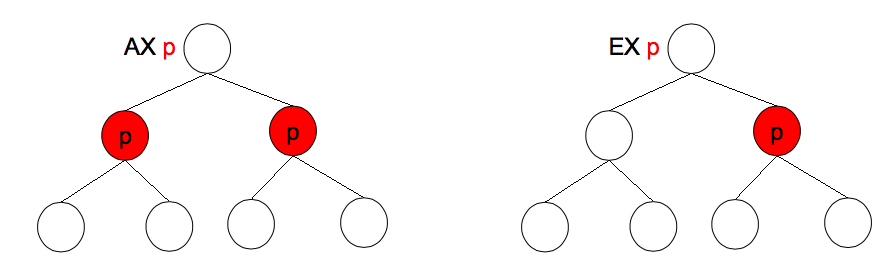
\includegraphics[width=130mm]{15/images/temporal}
\end{figure}
 % TVS
    %!TEX root=../oi-magistr-si.tex
\section[WA2 - Java EE]{Architektura Java EE, funkce jednotlivých vrstev, životní cyklus standardizovaných komponent Java EE, návrhové vzory využitelné v architektuře webové aplikace.}

Distribuce Javy se liší podle jejího zamýšleného použití:
\begin{itemize}[itemsep=0px]
\item \textbf{Java ME} (\textit{Java Micro Edition}) pro mobilní aplikace, omezený rozsah funkcí.
\item \textbf{Java SE} (\textit{Java Standard Edition}) pro desktopové aplikace.
\item \textbf{Java EE} (\textit{Java Enterprise Edition - J2EE}) pro webové aplikace.
\end{itemize}

\subsection{JAVA EE}
\begin{itemize}[itemsep=0px]
\item Komponentový přístup.
\item Komponenty mohou být distribuované na různých strojích (klient, server, DB).
\item Aplikace rozdělena do vrstev.
\item serverová část aplikace bývá nasazena na aplikačním serveru, který umožňuje zpracování více požadavků naráz (multi-threading). Nasazení znamená zabalení celého projektu do např. WAR archivu, který obsahuje vše potřebné (zdrojové třídy, statické resources, použité knihovny).
\item Podpora JNDI, java beans, JAAS (autentizace), JMS (Java Messaging Service), servlety, transakce (JTA – Java Transactions API).
\end{itemize}

\begin{figure}[h!]
\centering
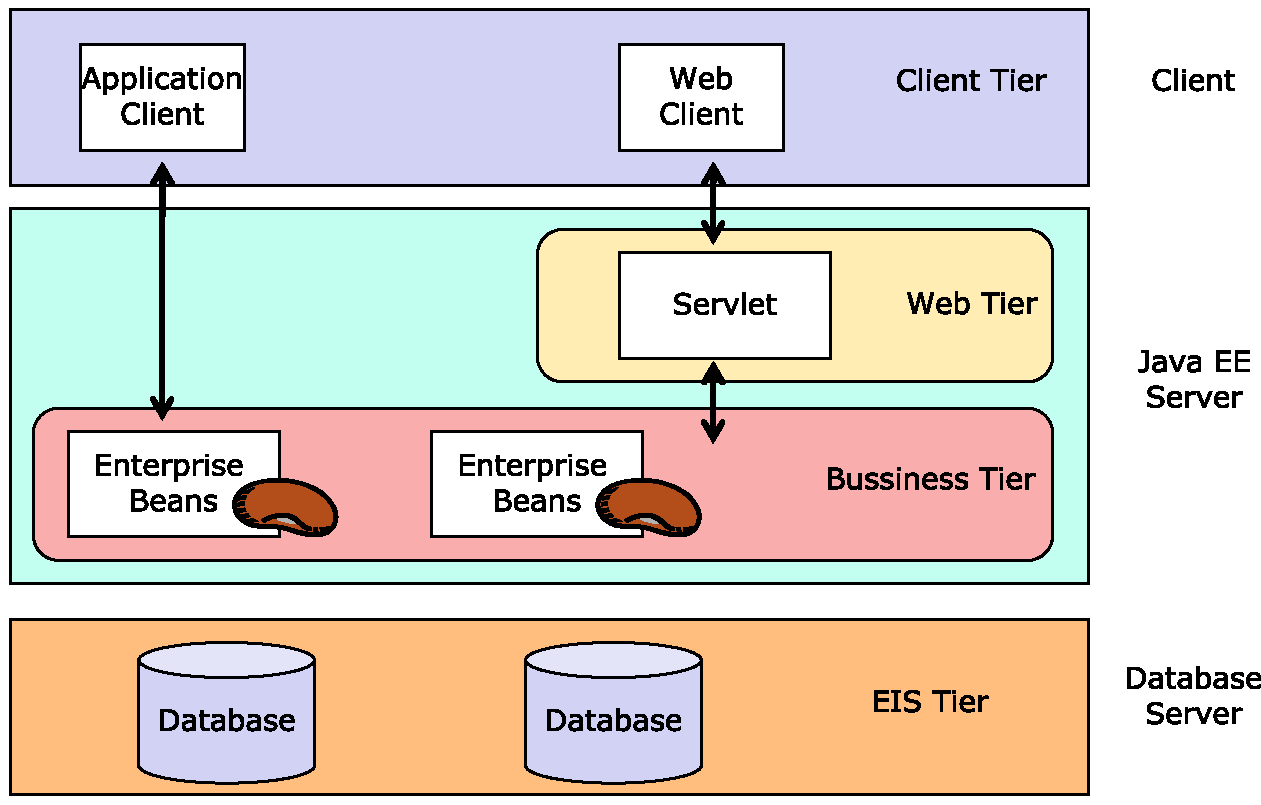
\includegraphics[width=140mm]{16/images/java-ee-arch}
\end{figure}

\paragraph{MVC} Většinou je aplikace navržena podle vzoru MVC. Jedná se o konkrétní aplikaci vzoru oddělení zodpovědností (\textit{separation of concerns}), který předepisuje vysokou kohezi jednotlivých komponent. Každá komponenta by měla mít vysoce soudržnou sadu zodpovědností a všechny ostatní požadavky by měla delegovat komponentám, které jsou úzce specializované zase na jinou činnost.

MVC tedy odděluje zodpovědnosti za data (model), pohled na data (view) a manipulaci s pohledem na data (controller). Aplikace je rozdělena na tři vrstvy: datovou, prezentační a ovladače (controllers). Tyto tři vrstvy jsou na sobě nezávislé a umožňují snadné vyjmutí jedné vrstvy a nahrazení jinou implementací.

\subsection{Servlet}
\textbf{Servlet je třída}, která rozšiřuje schopnost webserveru. \textbf{Zpracovává} a odpovídá na \textbf{požadavky} z webových klientů, typicky HTTP requestů. Třída musí implementovat rozhraní \texttt{javax.servlet.Servlet}, které definuje metody životní cyklu vyžadované servletovým kontejnerem. Při použití na webu servlet typicky rozšiřuje třídu \texttt{javax.servlet.http.HTTPServlet}, která definuje metody na zpracování jednotlivých HTTP požadavků: \texttt{doGet()}, \texttt{doPost()}, atd.

\begin{verbatim}
public class MujServlet extends HttpServlet { 
    @Override
    public void doGet(HttpServletRequest req, HttpServletResponse res) {
        res.getWriter().write("<html>Text ve formatu HTML</html>");
    }
}
\end{verbatim}

\paragraph{Životní cyklus} Aplikační server pro každý dotaz vytvoří nový servlet a zavolá nejdříve metodu \texttt{init()}. Pak následuje obsluha požadavku metodou \texttt{service()} a nakonec je po zavolání \texttt{destroy()} servlet zničen. Programátor může poskytnout vlastní implementaci metod \texttt{init()}, \texttt{service()} a \texttt{destroy()}.


\begin{figure}[h!]
\centering
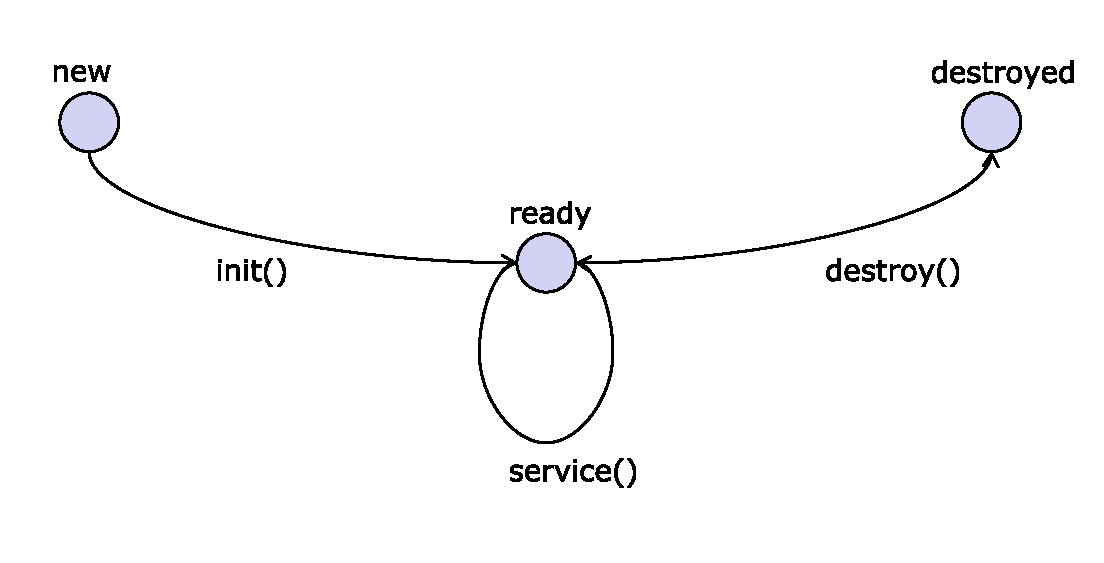
\includegraphics[width=80mm]{16/images/servlet-lifecycle}
\end{figure}

\vspace{-20px}

\paragraph{JSP (Java Server Pages)}
JSP je textový dokument obsahující statické (X)HTML tagy a JSP tagy, které umějí generovat dynamický obsah. JSP umožňuje používat kusy Java kódu v HTML stránce (scriptlet).

Za tím vším se ale skrývá servlet - \textbf{JSP jsou servlety}. JSP se při prvním použití kompiluje a vytvoří se Servlet, který dělá to, co uměla původní JSP stránka (např. do metody \texttt{doGet()} se \uv{vyprintí} celý obsah toho souboru).

\paragraph{Deskriptor} Deskriptor je konfigurační soubor s názvem \texttt{web.xml}, který musí být v každé webové aplikaci. Obsahuje mapování servletů a filtrů na requesty, kódování JSP stránek, parametry servletů a stanovuje, která stránka se zobrazí jako první (welcome-file).

\subsection{Java Bean}
Bean implementují aplikační logiku nebo vystupují v roli entit cílové domény (entita zákazník, výpůjčka...). Bean může mít lokální nebo vzdálené rozhraní podle toho, jestli ji se nachází na stejném stroji, nebo je na jiném stroji. Pak jsou také \textbf{EJB} (Enterprise Beans), to jsou komponenty běžící na aplikačním serveru, které jsou manažovány EJB kontejnerem. Bean je několik druhů:

\begin{itemize}[itemsep=0px]
\item \textbf{stateful} - Uchovává kontext pro každého klienta zvlášť. Je náročnější a pomalejší, proto bychom měli používat stateless, kdekoliv je to jen možné.
\item \textbf{stateless} - Jednodušší, nepamatuje si kontext volání klienta.
\item \textbf{message driven} - messaging (základní účel pro distribuované systémy).
\end{itemize}

\paragraph{Životní cyklus bean}

\begin{figure}[h!]
\centering
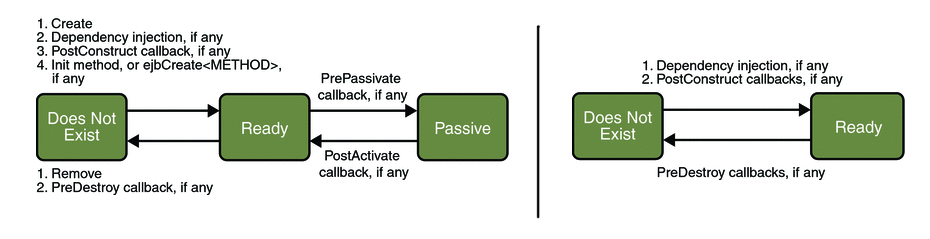
\includegraphics[width=140mm]{16/images/ejb-lifecycle}
\caption*{Životní cykly: stateful vs. stateless bean}
\end{figure}

\paragraph{Návrhové vzory využitelné v architektuře webové aplikace}
MVC, DI, Factory, Service Locator, cokoliv
 % WA2
    %!TEX root=../oi-magistr-si.tex
\section[WA2 - Web. architektury, perzistence, WS, messaging]{Vhodnost nasazení jednotlivých webových architektur, sdílení dat, perzistence, webové služby a REST, asynchronnost, messaging.}

\paragraph{Vhodnost nasazení jednotlivých webových architektur} záleží na povaze projektu. Třeba kalkulačka nemusí být vůbec na webu, eshop může běžet na vlastním serveru někde na hostingu u kamaráda, bankovní aplikace by měla mít tlustého i tenkého klienta a s použitím enterprise funkcí jako J2EE, server na sdílení videa bude chtít svůj privátní cloud aby dobře škáloval.

\priklad Elektronické bankovnictví, které má 20 let starý back-end legacy system naprogramovaný v COBOLu. Klienti přistupují přes webové JEE (JSP) rozhraní. zvážit architekturu systému vzhledem k nárůstu počtu klientů nebo růstu bank, zvážit privátní cloud vs. existující provideři AWS, Google, MS Azure.

Typická architektura (cloudové) aplikace. Je mnoho klientů, kteří interagují například s webovou službou. Ta může být horizontálně škálovatelná (co do počtu serverů). Zde může být i nějaký load balancer, který klienty rovnoměrně přiřazuje méně vytíženým strojům. Služba buď zpracuje požadavek rovnou do databáze (storage), nebo pokud se jedná o nějakou (časově) náročnější akci (například převod fotek atd.), tak tu pošle do fronty ke zpracování. Z fronty si tzv. \uv{worker role} postupně berou jednotlivé úlohy a na pozadí je provádění (opět mohou být horizontálně škálovatelné).

\begin{figure}[h!]
\centering
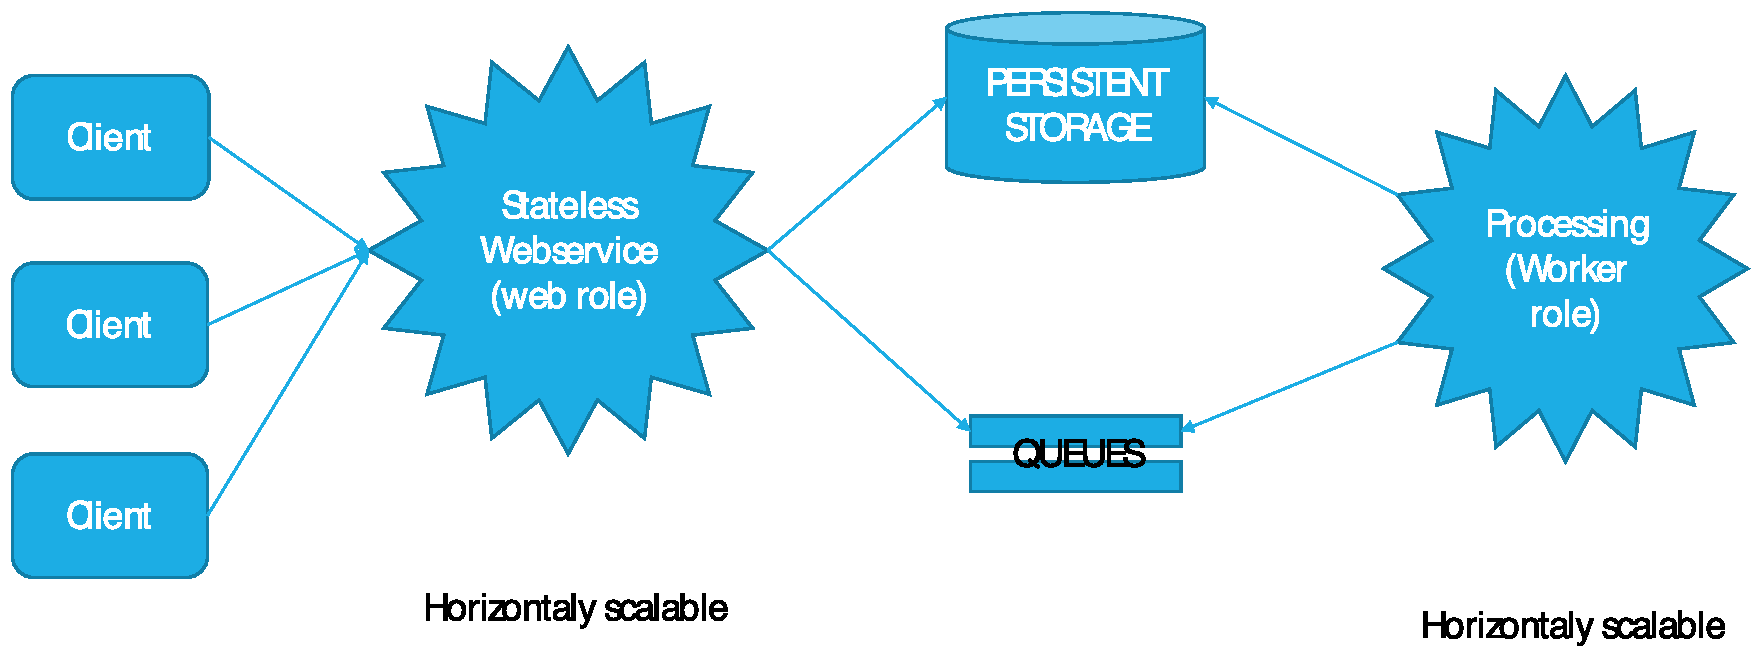
\includegraphics[width=130mm]{17/images/cloud-architecture}
\end{figure}

\subsection{Sdílení dat}
Master Slave vs. High replication

\subsection{persistence}
Hlavně relační DB, protože objektové nejsou moc cool - nevýhody přímého použití JDBC
\paragraph{ORM}
\begin{itemize}[itemsep=0px]
\item Blíže OO paradigmatu
\item JPA - standardizované API pro ORM: implementace např. Hibernate (konfigurace pomocí XML nebo anotacemi)
\item ORM by měl být neintruzivní - pracuje přímo s POJO (implicitní konstruktor, settery a gettery, ne final atributy)
\item podpora ISA (dědění) hierarchie:
    \begin{itemize}[itemsep=0px]
    \item SINGLE\_TABLE - vše v jedné tabulce + rozlišující sloupec
    \item TABLE\_PER\_CLASS - každá entita má vlastní tabulku s celou sadou atributů
    \item JOINED - hlavní tab. má základní attrib., ostatní se s ní spojují (slabé entity)
    \end{itemize}
\item podpora vztahů (1:1, 1:N, M:N)
\item dialekty SQL (snaha o sjednocení SQL syntaxe)
\item perzistenci se starají třídy EntityManager nebo Hibernate Session - operace \texttt{persist, find, merge, remove, query}
\end{itemize}

\subsection{WS a REST}
A web service is a function that can be accessed by other programs over the web (Http). A web service is a collection of open protocols and standards used for exchanging data between applications or systems. Software applications written in various programming languages and running on various platforms can use web services to exchange data over computer networks like the Internet in a manner similar to inter-process communication on a single computer. This interoperability (e.g., between Java and Python, or Windows and Linux applications) is due to the use of open standards (XML, SOAP, HTTP)

\begin{itemize}[itemsep=0px]
\item architektonický styl pro distribuovaná media
\item platformně nezávislé
\item založeno na technologii HTTP a URI
\item cíl: obecné aplikační rozhraní, možnost komunikace přes proxy - manipulace se zdroji (informace, data, soubory)
\item zdroj je identifikován svým URI
\item client-server (aplikační logika rozdělená mezi server a klient),
\item stateless (bezestavová komunikace - jeden požadavek nese všechny informace které server potřebuje k jeho zpracování),
\item pro popis metadat se používají HTTP hlavičky
\item minimalizace závislostí klienta a serveru
\item server může cacheovat odpovědi
\item klient neví, zda komunikuje se serverem nebo prostředníkem (proxy, cache)
\end{itemize}

\subsection{Messaging}
\noindent\textbf{Asynchronnost} znamená neblokující volání, dá se řešit třeba AJAXem nebo messagingem.

Messaging může efektivně řešit škálování a load balancing. Na serveru je fronta zpráv, kterou si rozebírají jednotlivé servery. Dá se využít na schedulování úkolů co trvají dlouho (konverze videa).

\textbf{JMS} (Java Messaging Service) dva módy: point-to-point (zprávy určené přímo někomu) nebo publish-subscribe (víc klientů se může subsribnout na nějaký topic)

\paragraph{Cloudové fronty:} GAE Task Queue, AWS SImple Queue Service, MS Azure Queue.

\begin{figure}[h!]
\centering
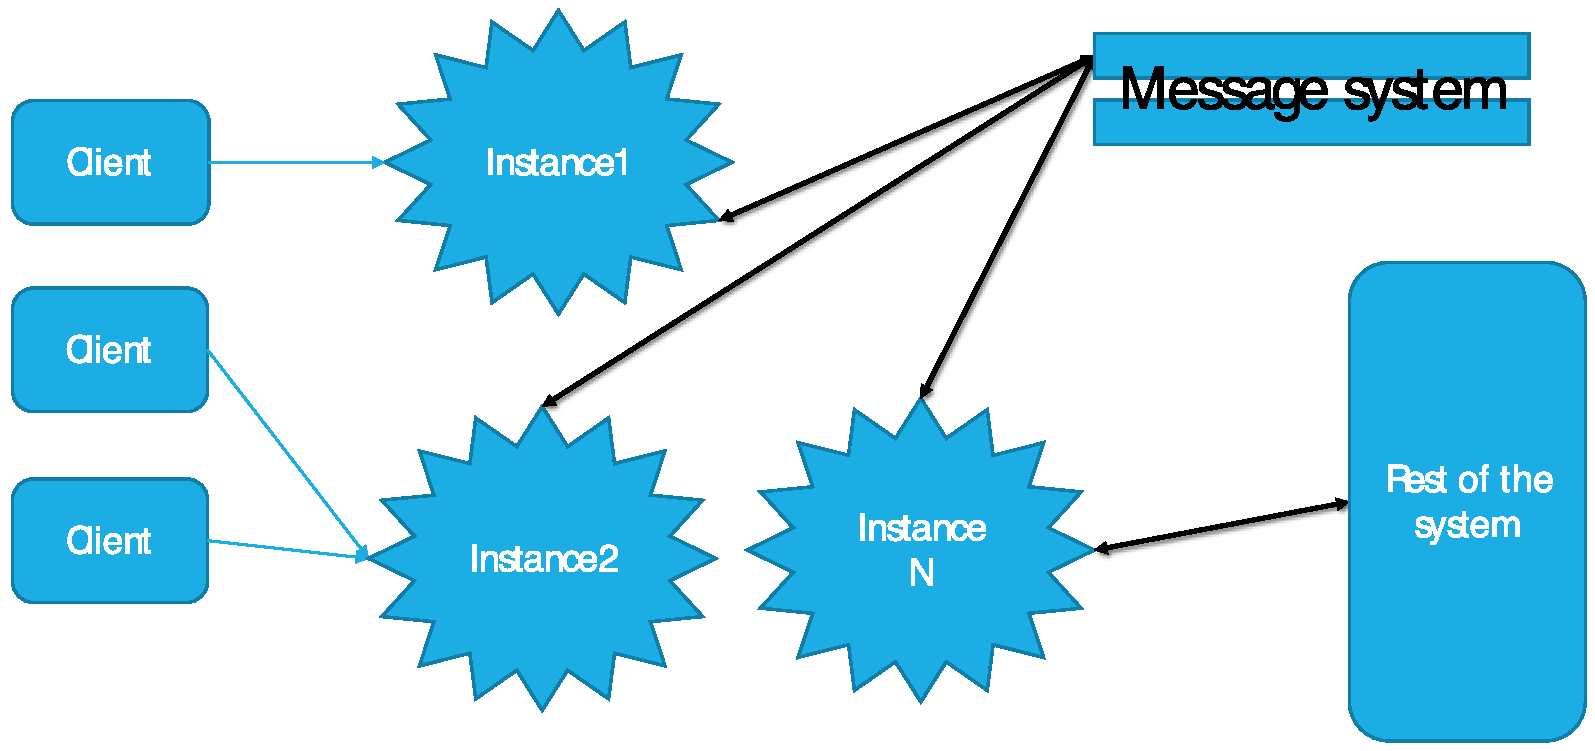
\includegraphics[width=140mm]{17/images/messaging}
\end{figure}
 % WA2
    %!TEX root=../oi-magistr-si.tex
\setcounter{section}{18}
\section[WA2 - Cloud]{Cloud architektury, virtualizace, různá pojetí cloudových řešení, omezení cloudových aplikací, náklady na provoz, vlastnosti aplikací vhodných pro nasazení v cloud architektuře.}

% https://docs.google.com/document/d/1v3kWgsxv67yEE10eLNGlU0HIaYy_OC1C5j8QX9k9ZSg/edit?hl=en_US#

Cloud-Computing architektury můžeme rozdělit do 3 hlavních vrstev:

\begin{figure}[h!]
\centering
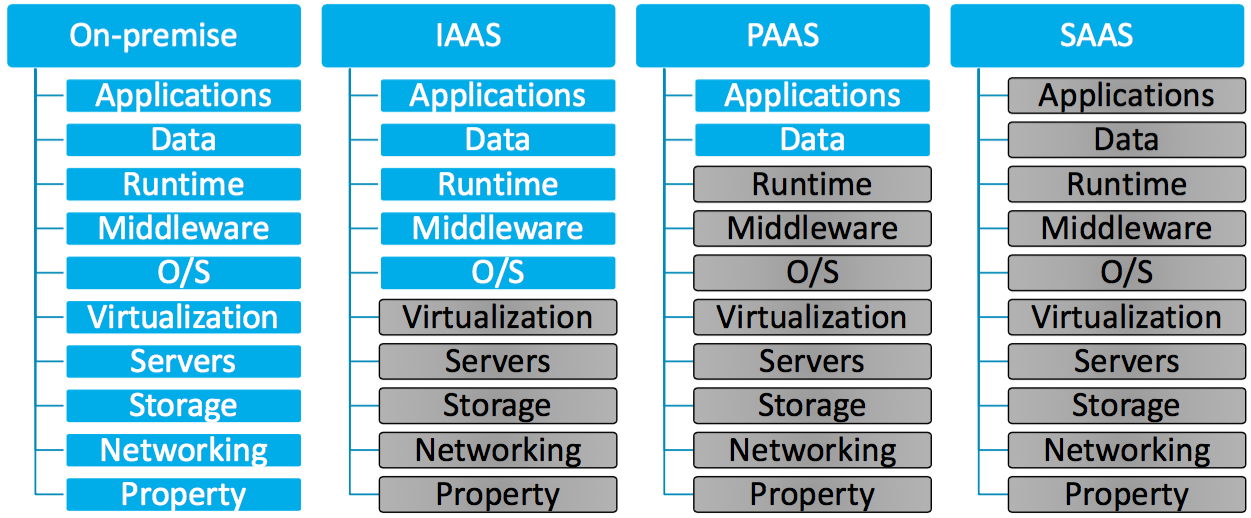
\includegraphics[width=140mm]{19/images/cloud-types}
\end{figure}


\subsection{Infrastructure as a Service (IaaS)}
Je to vlastně outsourcing výpočetního vybavení (servery, HW, síťové komponenty, storage). Poskytovatel služby je odpovědný za housing, běh a správu těchto komponent. Klient obvykle platí v modelu \textit{pay-as-you-go} či smluvním paušálem (předplatným), popřípadě kombinací obojího.
\paragraph{Příklady služeb IaaS:} Amazon EC2, Amazon S3, GTS Managed Server - Virtual Server.

\subsection{Platform as a Service (PaaS)}
Provider poskytuje přístup ke computing platformě či computing stacku (množina softwarových subsystemů, které poskládáte do výsledné služby). Jako v případě IaaS máte k dispozici servery, storage, ale omezené vybranou platformou. Zatímco na IaaS můžete v rámci virtuálního prostředí provozovat téměř jakoukoliv aplikaci, volba platformy (operacniho systemu ci programovaciho jazyka) je plně v kompetenci klienta, u PaaS jste již vázáni kompletní platformou.

\paragraph{Nebezpečí Vendor Lock-In} jste omezeni platformou poskytovate (.NET na MS Azzure), proprietární službou či množinou podporovaných programovacích jazyků. Flexibilita služby nemusí stačit rapidně se vyvyjejícím projektům (paměťové limity, model automatického deploymentu).

\paragraph{Příklady služeb PaaS} Google App Engine (platforma: Java, Python, Go), MS Azure (platforma: .NET, Ruby, Java, PHP).

\subsection{Software as a Service (SaaS)}
Model pronájmu hotových aplikací, které jsou k dispozici klientovi skrze interface (nejčastěji kombinace REST+JSON) či uživatelské rozhraní (Facebook, YouTube, BaseCampHQ, Google Apps.. ).
\paragraph{Příklady aplikací SaaS} Google Apps, E-mail, Kalendář, Microsoft Live

\subsection{Náklady na provoz}
\paragraph{Pay-As-You-Go} - Platíte pouze za spotřebované zdroje (použité storage, vypočetní čas, traffic). Obvykle 0 upfront investment. Konsolidovaná fakturace (denní, týdenní, .. vyúčtování za použité služby na jednom účtu). Cena zahrnuje náklady na:
\begin{itemize}[itemsep=0px]
\item hardware
\item údržba
\item utitilies
\item případné SW licence
\end{itemize}
Vendor uplatnuje obvykle economies-of-scale (jenotkove mensi naklady na MB storage, traffic, hodinu procesoroveho casu... )

\paragraph{Paušál} Můžete si předplatit určitý počet hodin procesorového času. Paušál za měsíční provoz virtual serveru atd..

\subsection{Virtualizace}
Emulace / Simulace 
VM simuluje cely HW. Vyuzitie: vyvoj a debug pre procesory, kt. su fyzicky nedostupne. 
Microsoft Virtual PC, emulator Hercula, AVD emulator pre Android
Nativni Virtualizace / Plna virtualizace
VM simuluje dostatocne mnozstvo HW, aby umoznilo oddeleny a bezpecny beh neupraveneho OS hosta
Virtual Box, Parallel Desktop
Castecna Virtualizace / virtualizace adresniho prostoru
VM simuluje viac instancii mnohych prostredi HW, na, ktorych bezi hostitel
Linux, MS Windows
Paravirtualizace
VM nesimuluje HW ale ponuka specialne API- “hypercall”, kt mozu byt vyuzite len z upraveneho hostovaneho OS.
Xenu, Parallel Workstations
Virtualizace na urovni OS
Umoznuje beh viacerych virtualych serverov na jednom fyzickom serveri. Virtualne servery maju rovnaky OS ako fyzicky.
Linux-VServer, Virtuozzo
Aplikacni Vritualizace
Vrstva mezi aplikaciou a OS
Java Virtual Machine, Citrix, VMware 
Virtualizace Backup
Forma: VLT (Virtual Tape Library) - zaznamenavalo sa na pasky 
VLT zariadenie simuluje princip mag. pasky. Najcastejsie vyuzivane medium - diskove pole rozdelene na casti, kt sa na vonok javia ako paskova mechanika
Forma: Deduplikace - virtualizacna technika kompresie dat, kt zabranuje ukladaniu rovnakych datovych blokov na jednom ulozisku -> uspora miesta
Virtualizace Storage 
Tenky (Thin) provisioning
virtualizacna technika umoznujuca prealokovat viac disk priestoru ako je fyzick mozne. (Zalozene na predpoklade ze aplikacie nevyuzivaju 100% alokovaneho miesta)
Automaticky Multitiering
automaticke presuvanie dat medzi vrstavmi podla ich vyuzitia (Tier1 - Fiber Channel - rychly/drahy, Tier2 - MidTier, Tier3 - Serial ATA - pomaly/lacny)



Sitova Virtualizace
WAN - Frame Relay
Technologia prepinania paketov WAN so schopnostou prisposobit prenajimanu sirku pasma. Vytvorene virtualne okruhy, kt mali min, gatrantovanu sirku pasma. Dnes sa uz nepouziva (umoznovala prenos dat aj hlasu)
WAN -VPN cez IP/MPLS - MultiProtocol Label Switching
smerovanie packetov v sieti na zaklade “lables” - rychlejsie ako vyhladavanie adresy v routovacich tabulkach. Umoznuje vznik VPN (Virtual Private Network)
LAN - VLAN (Virtual LAN)
technologia umoznuje vytvorenie nezaviclej siete v ramci jedneho alebo niekolkych zariadeni. Cielom je vytvorit logicku organizaciu siete nezavislu od fyzickej. Prinasa zvysenie vykonu, ulahcenie spravy siete, podpora bezpecnosti
Serverova virtualizacia
Prisla s mainframe-mami -> unixove servery -> dlho chybala na x86
(nic viac tam neviem dat -> doplnit ak ma niekto nieco)

Desktop Virtualizace
Ekonomicky výhodný způsob centrálního provozování aplikací a zpřístupnění dat – bezpečně a rychle
Standardizace, unifikace, soulad s normami
Získání zpět kontroly nad prací uživatele
Enterprise mobility – Doručení kamkoliv, kdykoliv, na čemkoliv - Bring Your Own Desktop

Nasadenie na cloud
Nasadenie existujucej aplikacie
	Treba sa zamysliet co je lepsie. Prekopat existujucu aplikaciu alebo postavit radsej novu? Na akom datovom ulozisku aplikacia bezi - potrebuje drahu relacnu databazu v cloude alebo Big Table, Blob? Riesit pomer cena vykon. Mam pouzit Iaas  (fund overhead na licencie ) alebo PaaS (hrozba vendor lock-in)

% Vlastnosti aplikací vhodných pro nasazení v cloud architektuře... dobře horizontálně škálovatelné (web. služby) % WA2

    \bibliographystyle{_lib/csplainnat}
    {
        \footnotesize
        \def\CS{$\cal C\kern-0.1667em\lower.5ex\hbox{$\cal S$}\kern-0.075em $}
        \bibliography{reference}
    }

\end{document}
